%%%%%%%%%%%%%%%%%%%%%%%%%%%%%%%%%%%%%%%%%%%%%%%%%%%%%%%%%%%%%%%%%%%%%%%%%%%%%%%%
% Where Exactly-Once Ends — RITA research article
% Based on the official RITA 2018 template (SelfArx.cls, archived official source;
% provenance and checksums in submission/VENUE-RULES.md).
% Compile: powershell -ExecutionPolicy Bypass -File build.ps1 -Main main.tex -Clean
%%%%%%%%%%%%%%%%%%%%%%%%%%%%%%%%%%%%%%%%%%%%%%%%%%%%%%%%%%%%%%%%%%%%%%%%%%%%%%%%

\documentclass[fleqn,12pt]{SelfArx} % 12 pt per written RITA guidelines (checklist); template class retained

%----------------------------------------------------------------------------------------
%	PACKAGES
%----------------------------------------------------------------------------------------
\usepackage[english]{babel}
\usepackage{url}
\usepackage{balance}
\usepackage{hyperref}
\usepackage{mathptmx}
\usepackage{graphicx}
\usepackage{times}
\usepackage{textcomp}
\usepackage{gensymb}
\usepackage{amsmath,amssymb}
\usepackage{comment}
\usepackage{multirow}
\usepackage[labelfont=bf]{subcaption}
\usepackage{booktabs}
\usepackage{enumitem}
\usepackage{tcolorbox}
\usepackage[num]{abntex2cite}
\citebrackets[]
\usepackage{tikz}
\usetikzlibrary{arrows.meta,positioning,shapes.geometric,calc}
\usepackage{algorithm}
\usepackage{algpseudocode}
\usepackage{amsthm}

% Theorem environments for the formal part (author-owned content, drafted by the team)
\theoremstyle{plain}
\newtheorem{proposition}{Proposition}
\newtheorem{lemma}{Lemma}
\newtheorem{theorem}{Theorem}
\newtheorem{corollary}{Corollary}
\theoremstyle{definition}
\newtheorem{definition}{Definition}
\newtheorem{assumption}{Assumption}

% Manuscript/analysis integration: analysis outputs (owned by S4) define these if present.
\inputifexists{results/analysis/macros.tex}
\providecommand{\ResHypothesisOneVerdict}{pending}
\providecommand{\ResHypothesisTwoVerdict}{pending}
\providecommand{\ResHypothesisThreeVerdict}{pending}
\providecommand{\ResHypothesisFourVerdict}{pending}
\providecommand{\ResHypothesisFiveVerdict}{pending}
\providecommand{\ResTotalValidRuns}{--}
\providecommand{\ResTotalExcludedRuns}{--}
\providecommand{\ResMzeroViolatingRuns}{--}
\providecommand{\ResMzeroViolationRate}{--}
\providecommand{\ResMonexViolatingRuns}{--}
\providecommand{\ResMonexViolationRate}{--}
\providecommand{\ResMtwoViolatingRuns}{--}
\providecommand{\ResMthreeViolatingRuns}{--}
\providecommand{\ResMfourViolatingRuns}{--}
\providecommand{\ResMtwoPlusMthreeViolatingRuns}{--}
\providecommand{\ResMfourPlusMthreeViolatingRuns}{--}
\providecommand{\ResMonexPlusMthreeViolatingRuns}{--}
\providecommand{\ResMkafkaViolatingRuns}{--}
\providecommand{\ResEarlyProbeLossRuns}{--}
\providecommand{\ResSubstrateDeviationText}{native Windows processes instead of containers}
\newcommand{\code}[1]{\texttt{#1}}
\newcommand{\inputifexists}[1]{\IfFileExists{#1}{\input{#1}}{}}

% RITA template rule colour / boxes
\definecolor{mycolor}{rgb}{0,0,0}
\makeatletter
\newcommand{\mybox}[1]{%
	\setbox0=\hbox{#1}%
	\setlength{\@tempdima}{\dimexpr\wd0+13pt}%
	\begin{tcolorbox}[colframe=mycolor,boxrule=0.5pt,arc=4pt,
		left=6pt,right=6pt,top=6pt,bottom=6pt,boxsep=0pt,width=\@tempdima]
		#1
	\end{tcolorbox}
}
\makeatother

%----------------------------------------------------------------------------------------
%	COLUMNS AND COLOURS (as in the official template)
%----------------------------------------------------------------------------------------
\setlength{\columnsep}{0.55cm}
\setlength{\fboxrule}{0.75pt}
\definecolor{color1}{RGB}{0,0,90}
\definecolor{color2}{RGB}{0,20,20}

\hypersetup{hidelinks,colorlinks,breaklinks=true,urlcolor=color2,citecolor=color1,linkcolor=color1,
bookmarksopen=false,pdftitle={Where Exactly-Once Ends},pdfauthor={Joao Brito}}

%----------------------------------------------------------------------------------------
%	ARTICLE INFORMATION
%----------------------------------------------------------------------------------------
\JournalInfo{\color{gray}\normalsize\sffamily\bfseries Revista de Informática Teórica e Aplicada - RITA - ISSN 2175-2745\\ Vol.~XX, Num.~XX~(2026)~1-XX}
\Archive{\mybox{RESEARCH ARTICLE}}

\PaperTitle{Where Exactly-Once Ends: Preserving Double-Entry Ledger Invariants When Apache Kafka Pipelines Write to External Stores}
\ShortTitle{Where Exactly-Once Ends}

\Titulo{Onde o Exactly-Once Termina: Preservando Invariantes de Razão de Dupla Entrada Quando Pipelines Apache Kafka Escrevem em Armazenamentos Externos}

\PaperVol{XX}
\PaperNum{X}
\PaperAno{2026}

\Authors{João Brito\textsuperscript{1,*}}
\affiliation{\textsuperscript{1}\textit{Universidade Federal do ABC (UFABC), Santo André, SP, Brazil}}
\affiliation{*\textbf{Corresponding author}: correiadebrito.joao@gmail.com}

\Keywords{Exactly-once semantics --- Apache Kafka --- double-entry ledger --- transactional outbox --- idempotency --- fault injection}
\newcommand{\keywordname}{Keywords}
\PalavrasChave{Semântica exactly-once --- Apache Kafka --- razão de dupla entrada --- outbox transacional --- idempotência --- injeção de falhas}

\Doi{http://dx.doi.org/10.22456/2175-2745.XXXX}
\DateR{dd/mm/yyyy}
\DateA{dd/mm/yyyy}

%----------------------------------------------------------------------------------------
%	ABSTRACT (<= 200 words) — PENDING final results; placeholder kept explicit for build tests
%----------------------------------------------------------------------------------------
\Abstract{PLACEHOLDER ABSTRACT (to be replaced after results): this paper studies where Apache Kafka's exactly-once semantics ends when a pipeline's side effect must land in an external relational database, and what that boundary means for double-entry ledger invariants. We formalise the ledger state machine, define the EOS boundary, and give invariant-preservation arguments or counterexamples for five mechanisms (naive at-least-once, Kafka EOS with internal and external sinks, transactional outbox, idempotency keys with a unique index, and database-resident offsets) and three combinations under six scripted fault modes. An independent oracle measures duplicate and lost postings, invariant violations, throughput and tail latency across a staged experiment matrix.}

\Resumo{RESUMO PROVISÓRIO (a ser substituído após os resultados): este artigo estuda onde termina a semântica exactly-once do Apache Kafka quando o efeito colateral de um pipeline precisa ser gravado em um banco de dados relacional externo e o que esse limite significa para invariantes de razão de dupla entrada. Formalizamos a máquina de estados do livro-razão, definimos a fronteira EOS e apresentamos argumentos de preservação de invariantes ou contraexemplos para cinco mecanismos e três combinações sob seis modos de falha roteirizados. Um oráculo independente mede lançamentos duplicados e perdidos, violações de invariantes, vazão e latência de cauda em uma matriz experimental escalonada.}

%----------------------------------------------------------------------------------------
\begin{document}
\setcounter{page}{1}
\flushbottom
\maketitle
\thispagestyle{empty}

% Section 1 — Introduction
% Drafted by the lead from docs/method.md, docs/AMENDMENT-A1.md and the verified reference base.
% No result values appear here: outcome-dependent sentences live in Section 7.

\section{Introduction}
\label{sec:intro}

Event-driven architectures have become the default way to move money between financial
institutions. A payment is ingested as an event, validated, split into debit and credit legs, and
appended to a general ledger; downstream services notify counterparties, update balances, and
trigger settlement. Apache Kafka is the most common substrate for this pipeline, and its
\emph{exactly-once semantics} (EOS) is routinely presented as the guarantee that makes the
pipeline safe: a record is said to be processed exactly once even in the presence of broker
failures, consumer crashes and rebalances~\cite{kip98,kafka-design}.

The guarantee is real, but bounded. Kafka's transactions make \emph{Kafka-internal} effects
atomic: records appended to Kafka topics, consumer offsets committed through the transaction
coordinator, and the producer's own idempotency state all commit or abort together. When the
useful side effect of the computation must land in an external system --- a PostgreSQL ledger, a
core-banking database, a payment rail --- that write is a separate transaction at a separate site,
with its own write-ahead log and no shared coordinator. Kafka's own documentation is explicit that
in this case the consumer's position must be coordinated with what is actually stored as
output~\cite{kafka-design}; the exactly-once guarantee is not a distributed transaction spanning
Kafka and the external store~\cite{kip98,txncommit2006}.

For most applications the resulting duplicates or gaps are an annoyance to be cleaned up later. In
a double-entry ledger they are a correctness failure of a different kind. Accounting represents
every economic event as a journal entry whose debit and credit legs sum to zero, and it requires
that the ledger be append-only and that each business event appear exactly once. A duplicate
posting is not a redundant row that can be deleted in a reconciliation job without breaking
auditability: it silently changes balances, often in a way that still sums to zero and therefore
passes naive balance checks. A lost posting is worse: the money exists on one side of the books
only, and no later retry can be distinguished from a legitimate new event unless the pipeline
carried an idempotency mechanism. Both failures are silent, permanent, and exactly the kind of
defect that surfaced in industrial incident reports and in the correctness discussions around
streaming data pipelines~\cite{kafka2015,flink2017,bailis2014}.

Practitioners nevertheless deploy pipelines in which Kafka transactions are treated as if they
covered the database write. The pattern has a long history: an application consumes a record,
writes to the database, and then commits the offset inside a Kafka transaction (or, in older
Spring code, inside a ``chained'' transaction manager), with the implicit assumption that either
both commits happen or neither does. When the process dies between the two commits, or when one
commit succeeds while the other times out, the assumption fails. What is missing from the
literature is not the theoretical observation that two sites cannot be committed atomically
without a protocol such as two-phase commit~\cite{txncommit2006,pg-prepare}, but a systematic,
empirical mapping from failure modes to ledger-invariant violations, mechanism by mechanism, with
the cost of each remedy measured under the same conditions. Survey work on microservice data
consistency documents the patterns and the practitioner confusion but reports no fault-injection
counts~\cite{laigner2021,micro2026}; systems papers on exactly-once semantics stop at the
framework's own state~\cite{flink2017,millwheel2013,dstreams2013}; and ledger/auditability work
assumes the invariant rather than testing its preservation~\cite{triple2019,triple2021}.

This paper closes that gap for the canonical case: a Kafka source topic whose records are
balanced journal entries, a consumer service that must append the corresponding postings to an
external relational database and maintain consumption progress, and a pipeline that must keep
four ledger invariants under scripted faults. We ask three questions.
\textbf{RQ1:} for which failure modes does Kafka EOS fail to preserve double-entry ledger
invariants when the sink is an external relational database?
\textbf{RQ2:} how do five mechanisms and three combinations compare --- naive at-least-once
(M0, negative control), Kafka EOS with a Kafka-internal sink (M1-kafka, positive control), Kafka
EOS wrapped around a non-atomic external write (M1x, the deployed pattern), a transactional
outbox/inbox (M2), idempotency keys with a unique index (M3), offsets stored in the ledger
database transaction (M4), and M2+M3, M4+M3, M1x+M3 --- on duplicate postings, lost postings,
invariant violations, throughput and tail latency?
\textbf{RQ3:} what is the minimal mechanism set sufficient for each failure-exposure class?

Our approach has four components. First, we define the ledger state machine and the precise
\emph{EOS boundary} of the pipeline, enumerate every point at which a process can crash or a
message can be lost, duplicated or reordered (crash points C1--C12), and give an
invariant-preservation proposition or an explicit counterexample trace for every mechanism and
crash-point class. A bounded version of the crash-point semantics is machine-checked with TLC,
which confirms the expected duplicate and loss witnesses within stated bounds; the model is a
bounded witness, not an unbounded proof, and we are explicit about the difference. Second, we
implement all nine configurations in one code base with identical tuning, and inject six fault
modes with real scripted injectors --- broker kills, consumer kills, produce timeouts with unknown
outcome, commit-order failures in both directions, database network partitions, and duplicate
redelivery after rebalance --- alongside deterministic crash-point failpoints. Third, we score
every run with an independent oracle: the load generator writes the expected posting set before
producing, and a separate Python checker recomputes it from the specification and compares it with
the database after quiescence, so duplicates, losses, imbalance and mutation are measured rather
than inferred from logs. Fourth, we pre-register the statistical analysis plan (exact confidence
intervals for mostly-zero correctness outcomes, bootstrap intervals and Friedman/Nemenyi/Cliff's
delta for performance) and execute a staged campaign designed to fit a fixed wall-clock budget,
recording every deviation.

Our contributions are:
\begin{itemize}[leftmargin=1.1em,itemsep=1pt]
\item a formal ledger and EOS-boundary model with a crash-point enumeration and
      invariant-preservation propositions for nine mechanism configurations, including a
      machine-checked bounded TLC model of the duplicate (W1) and loss (W2) windows;
\item the first fault-injection comparison, to our knowledge, of EOS-boundary mechanisms scored
      directly on double-entry invariants with an independent oracle and pre-registered statistics;
\item a practitioner decision table mapping failure exposure to the minimal sufficient mechanism
      set, with the measured cost of each additional guarantee;
\item a public, reproducible artifact containing the service, the fault injectors, the oracle,
      the raw run records and the scripts that regenerate every table and figure.
\end{itemize}

The remainder of the paper is organised as follows. Section~\ref{sec:related} reviews Kafka EOS,
consistency mechanisms, ledger invariants and experimental methodology. Section~\ref{sec:model}
defines the system, ledger state machine, invariants and the EOS boundary.
Section~\ref{sec:mechanisms} presents the mechanisms. Section~\ref{sec:formal} states and argues
the invariant-preservation results and reports the machine-checked model.
Section~\ref{sec:method} describes the implementation, faults, oracle and pre-registered design.
Section~\ref{sec:results} reports correctness and performance results and the hypothesis verdicts.
Section~\ref{sec:decision} derives the decision table, Section~\ref{sec:threats} discusses threats
to validity, and Section~\ref{sec:conclusion} concludes.


% Section 2 — Background and Related Work (compressed per compliance plan; all claims retained)
\section{Background and Related Work}
\label{sec:related}

\subsection{Kafka exactly-once and stream-processing fault tolerance}
\label{sec:rel-eos}

Kafka is a replicated, partitioned commit log with per-partition ordering~\cite{kafka2015}. Its
transactional API (KIP-98) adds a coordinator, producer epoch and transaction log so a producer
can atomically append records across partitions and commit offsets in the same
transaction~\cite{kip98,kafka-design}. The guarantee is producer-scoped: it covers Kafka's own
durable state, not arbitrary external effects. Fencing by \code{transactional.id} (KIP-447)
invalidates zombie producers~\cite{kip447}, and incremental cooperative rebalancing (KIP-429)
changes when offsets are committed~\cite{kip429}.

Stream-processing systems reached the same conclusion earlier: fault tolerance is built
around consistent snapshots of \emph{internal} state. MillWheel places timers and state
under its own envelope~\cite{millwheel2013}; Flink snapshots state without stopping the
pipeline~\cite{flink2017}; Spark Streaming recovers lineage-based
state~\cite{dstreams2013}; timely dataflow coordinates by logical
timestamps~\cite{naiad2013}. The theoretical basis is the distributed snapshot of Chandy
and Lamport~\cite{chandy1985}, and the stream/table duality frames a materialised view as
a stream of updates~\cite{sax2018}. Dataflow's model makes the correctness--latency--cost
trade-off explicit~\cite{dataflow2015}. None of these frameworks makes an unrelated
external database commit part of its snapshot; the external sink is outside the envelope,
which is precisely the boundary this paper measures.

\subsection{Transactions, idempotency and consistency}
\label{sec:rel-txn}

Across two sites, atomic commitment needs a protocol: two-phase commit blocks if its coordinator
fails, which motivates consensus-based commit and compensating approaches~\cite{txncommit2006,pg-prepare}.
Sagas replace atomic commit with local transactions and compensations and restore eventual
consistency, but not a duplicate-free ledger, because compensations are observable intermediate
states~\cite{sagas1987,saga2022}. Isolation levels are defined by the anomalies they permit, and
several ANSI levels allow the lost-update and dirty-read phenomena that would make an
independently committed ledger row unreliable~\cite{berenson1995,pg-isolation}. Coordination can
be avoided only when invariants are confluent~\cite{bailis2014}; the ledger's one-entry-per-event
requirement is not confluent with an at-least-once source, which is why the mechanisms of
Section~\ref{sec:mechanisms} must add idempotency, atomic progress or both. Optimistic
concurrency and reliability engineering supply the classical tools~\cite{kung1981,vogels2009}.

Idempotency is the second classical answer. Exactly-once delivery has been studied in
messaging middleware~\cite{eosmsg2001,eosmid2012}, and request identifiers that survive
crashes deduplicate retried CORBA-era invocations~\cite{eoscorba1999}. Modern APIs expose
idempotency keys~\cite{stripe-idempotency}, and relational engines enforce
them with a unique constraint and \code{ON CONFLICT DO NOTHING}~\cite{pg-onconflict}. The
subtlety isolated here is that deduplication and loss are different failures: a key makes
a retry harmless but cannot restore an effect never written before progress advanced.

\subsection{Microservice data patterns and the outbox}
\label{sec:rel-micro}

The transactional outbox publishes database changes by writing the outgoing message in the same
local transaction and relaying it afterwards~\cite{debezium-outbox}; event sourcing and CQRS
build the application from an ordered event log~\cite{eventsourcing2022}; saga frameworks supply
compensation orchestration~\cite{saga2019,saga2022}. Surveys document the pattern landscape and
the absence of a shared consistency definition, but report no fault-injection
measurements~\cite{laigner2021,micro2026}. Our M2 is the consumer-side dual of the outbox: an
inbox claim plus a publication log inside the ledger transaction, with a relay making publication
recoverable.

\subsection{Double-entry ledgers, append-only state and logical order}
\label{sec:rel-ledger}

Double-entry bookkeeping is a six-century-old invariant-bearing model: debits equal
credits and the ledger is append-only. Triple-entry accounting adds an externally
auditable record of each entry~\cite{triple2019,triple2021}. The systems substrate for
such a record is the log-structured store, whose append-only discipline bounds
corruption~\cite{lsfs1992}, together with logical clocks that totally order
events~\cite{lamport1978}. Our ledger model in Section~\ref{sec:model} is deliberately
small --- one currency, balanced two-leg entries, append-only postings --- but faithful to
the invariants that distinguish a ledger from a generic table, and the oracle tests them
directly.

\subsection{Formal specification and verification}
\label{sec:rel-formal}

We use TLA+ to state the crash-point semantics and machine-check a bounded version of the
preservation claims~\cite{lamport1994}; Alloy's analysis of structural constraints is
complementary for data-model reasoning~\cite{jackson2002}. Verified distributed systems
make the fault model explicit, most prominently in Verdi~\cite{verdi2015}. We follow that
discipline: assumptions (crash-recovery, no Byzantine faults, a fixed isolation level, one
host) are stated in Section~\ref{sec:model}, and the TLC check in
Section~\ref{sec:formal} is reported with its bounds so it cannot be mistaken for an
unbounded proof.

\subsection{Measurement, fault injection and statistics}
\label{sec:rel-method}

Benchmarking fault-tolerant systems requires care. Hoefler and Belli survey sound reporting
practice~\cite{hoefler2015}; Raasveldt et al.\ catalogue fairness pitfalls~\cite{raasveldt2018};
Mytkowicz et al.\ show measurement bias alone can reverse conclusions~\cite{mytkowicz2009};
Dean and Barroso explain why tail latency dominates responsiveness~\cite{dean2013}; Theodolite
demonstrates use-case-based scalability benchmarking~\cite{theodolite2021}. We therefore fix all
non-mechanism configuration identically, randomise and interleave run order, use paired seeds,
and report open-loop distributions with HdrHistogram.

Fault injection is our independent variable. Chaos engineering frames hypothesis-driven
experiments against a steady state~\cite{basiri2016}; black-box history checking exposes
isolation anomalies~\cite{elle2020}; deterministic simulation tests features under many
faults~\cite{fdb2021}; bounded crash testing found bugs even in verified
systems~\cite{crashmonkey2019}; repeatability requires archived data~\cite{collberg2016}. Our
injectors act on real processes and real TCP links Toxiproxy and write a
timestamped receipt, so a run whose fault did not fire is excluded, not counted as evidence.

Our analysis plan follows the experimental-statistics literature: randomised and benchmark
comparisons need appropriate tests~\cite{arcuri2011,arcuri2012}; multiple comparisons call
for Friedman and Nemenyi procedures~\cite{demsar2006}; paired proportions use McNemar's
test~\cite{mcnemar1947} with Holm's correction~\cite{holland1987}; effect sizes use
Cliff's delta~\cite{cliff1993}; interval estimates use the bootstrap~\cite{efron1979};
binomial intervals for mostly-zero violation counts use Clopper--Pearson
constructions~\cite{jsta2014,brown2001} and the rule of three for zero-event
bounds~\cite{rule3}.

\subsection{Research gap}
\label{sec:rel-gap}

The literature establishes three facts: Kafka EOS is bounded to Kafka's own state; external
state requires an explicit mechanism; and ledger invariants are unforgiving of duplicates
and losses. What is missing is an empirical, mechanism-level mapping from failure modes to
ledger-invariant violations, with an independent oracle and the cost of each remedy measured
under identical conditions. The closest practitioner-facing statements are vendor
documentation~\cite{kafka-design,debezium-outbox,stripe-idempotency} and microservice
surveys~\cite{laigner2021,micro2026}, neither of which measures invariant violations under
injected faults. This paper provides that mapping, its formal basis, and a decision
procedure for practitioners.


% ============================================================================
% sections/system.tex -- Section 3: System and Failure Model
% Drafted from the P1-approved docs/method.md (§1.3--§1.5, §2, §3).
% ============================================================================

% Theorem-like environments. Defined once here (guarded, so a later preamble
% addition cannot clash); base-LaTeX \newtheorem is used because amsthm is not
% loaded by the class.
\makeatletter
\@ifundefined{c@proposition}{\newtheorem{proposition}{Proposition}}{}
\@ifundefined{c@lemma}{\newtheorem{lemma}{Lemma}}{}
\@ifundefined{c@corollary}{\newtheorem{corollary}{Corollary}}{}
\@ifundefined{proofsketch}{%
  \newenvironment{proofsketch}{\par\noindent\emph{Proof sketch.}\ }{\hfill$\square$\par}}{}
\makeatother

\section{System and Failure Model}
\label{sec:model}

This section fixes the vocabulary used throughout the paper: the pipeline and its
durable stores, the event and ledger schemas, the ledger invariants, the boundary of
Kafka's exactly-once guarantee, and the crash-point model against which the mechanisms
are analysed.

\subsection{Pipeline and durable stores}
\label{sec:model:pipeline}

The pipeline is the canonical form of a ledger ingestion service: a Kafka source topic
carries business events; a consumer service applies a deterministic function to each
record and performs two durable side effects; a load generator produces the events and
an independent oracle verifies the end state. Kafka is used as a replicated,
partitioned log \cite{kafka2015}; the source topic is partitioned, replicated with
factor three and consumed by a consumer group whose offsets are committed to Kafka's
offset store. The consumer group is the unit of progress; partitions are the unit of
parallelism.

Two durable stores receive side effects. The first is the \emph{ledger sink}: a
PostgreSQL database whose posting table is the authoritative record of the ledger. The
second is the \emph{publication stream}: a Kafka topic to which one derived entry record
per business event is appended, used by downstream audit consumers
\cite{sax2018,eventsourcing2022}. For the DB-sink mechanisms (M0, M1x, M2, M3, M4 and
the combinations) the ledger is PostgreSQL and the publication stream is auxiliary; for
the Kafka-sink mechanism (M1-kafka) the publication stream \emph{is} the ledger. This
distinction is a construct-validity matter and is stated wherever mechanisms are
compared (Section~\ref{sec:mechanisms}).

The deployment analysed here is deliberately modest and reproducible: three Kafka
KRaft broker processes, one PostgreSQL instance, one Toxiproxy process for TCP faults,
and the consumer service at two instances in one consumer group. Table~\ref{tab:components}
lists the components and their failure-relevant roles. The single-host deployment is a
fidelity limitation discussed in the threats-to-validity section; it is not a modelling
simplification: the mechanisms are the ones deployed in practice, and every fault is a
real process kill or a real TCP manipulation, not a simulation.

\begin{table*}[t]
\centering
\small
\caption{Executed system: components, roles, and failure-relevant properties. All
components are native processes; the substrate and version pinning are described in
Section~\ref{sec:method}.}
\label{tab:components}
\begin{tabular}{@{}p{2.6cm}p{2.2cm}p{6.2cm}p{4.2cm}@{}}
\toprule
Component & Instances & Role & Durable state \\
\midrule
Kafka brokers (KRaft) & 3 & replicated source log, publication stream, consumer offsets, transaction state & log segments, offset store, transaction state \\
PostgreSQL 16 & 1 & authoritative ledger for DB-sink mechanisms; progress, inbox and outbox tables where the mechanism uses them & ledger tables, progress tables, WAL \\
Consumer service & 2 & one instance of the mechanism under test; reads source records and performs the mechanism's durable duties & none of its own (recovery uses the mechanism's durable state) \\
Load generator & 1 & deterministic open-loop producer; writes ground truth before producing & ground-truth file and produced manifest \\
Toxiproxy & 1 & cuts, delays and resets real TCP connections (app$\leftrightarrow$Kafka, app$\leftrightarrow$PostgreSQL) & none \\
Runner and injectors & 1 & per-run orchestration, fault injection, fault attestation, run records & run records and fault log \\
Oracle & 1 & independent verifier: re-derives the expected postings and compares them with the sink & analysis output only \\
\bottomrule
\end{tabular}
\end{table*}

\subsection{Events, entries, and postings}
\label{sec:model:schema}

One source record carries exactly one complete journal entry: a business event
$e=(\mathit{eid},\mathit{cur},\mathit{legs})$ with $\mathit{legs}=((a_D,D,m),(a_C,C,m))$,
$m\in\mathbb{Z}^{+}$ and $a_D\neq a_C$. The two legs are one debit (D) of $m$ minor
units and one credit (C) of the same amount in the same currency. The restriction to
two-leg, single-currency entries is a scoping decision: it keeps the unit of atomicity
at the record level and isolates the external-store boundary, which is the object of
study; multi-leg and multi-currency entries are not modelled
(Section~\ref{sec:model:assumptions}, assumption A12).

Events are a pure function of a per-repetition seed and a global sequence number: the
$\mathit{eid}$, both account identifiers, the amount and the target partition are
derived with SHA-256 over domain-separated inputs. The generator and the oracle
implement the same derivation independently, so the expected posting set is
recomputable rather than stored, and the two implementations can be compared
byte-for-byte. This is the mechanism behind the independent oracle of
Section~\ref{sec:method}.

The ledger sink stores \emph{postings}, one row per leg. Table~\ref{tab:posting}
summarises the schema. Postings are append-only: the application role holds only
\texttt{INSERT} and \texttt{SELECT} on the table, and a trigger rejects every
\texttt{UPDATE} or \texttt{DELETE}. The deduplication index on
$(\mathit{event\_id},\mathit{leg\_no})$ exists only in mechanisms that use
de-duplication; its absence in the naive mechanisms is part of the treatment, not an
implementation accident. Amounts are integers in minor units; no floating point
appears in the pipeline.

\begin{table}[t]
\centering
\small
\caption{Ledger sink schema (columns abbreviated). The unique index is present only in
the de-duplicating mechanisms (M3, M2+M3, M4+M3, M1x+M3). Append-only enforcement is
identical for all mechanisms.}
\label{tab:posting}
\begin{tabular}{@{}p{2.9cm}p{1.8cm}p{2.4cm}@{}}
\toprule
Column & Type & Constraint \\
\midrule
\texttt{posting\_id} & bigserial & primary key \\
\texttt{event\_id} & text & not null \\
\texttt{leg\_no} & smallint & check $\in\{1,2\}$ \\
\texttt{account\_id} & text & not null \\
\texttt{side} & char(1) & check $\in\{\mathrm{D},\mathrm{C}\}$ \\
\texttt{amount\_minor} & bigint & check $>0$ \\
\texttt{currency} & char(3) & not null \\
\texttt{produced\_at} & timestamptz & from the event \\
\midrule
\multicolumn{3}{@{}p{7.1cm}@{}}{\texttt{UNIQUE(event\_id, leg\_no)} --- de-duplicating mechanisms only} \\
\bottomrule
\end{tabular}
\end{table}

\subsection{Ledger invariants and observation}
\label{sec:model:invariants}

A ledger is correct when it records every consumed business event exactly once and no
other posting. Double-entry bookkeeping requires each entry to be balanced
\cite{triple2019,triple2021}; append-only recording is the classic durability
discipline for journals \cite{lsfs1992}. We therefore identify four invariants. Let
$D$ be the observed posting multiset (rows of the sink, or committed records of the
publication stream when that stream is the ledger) and let $\Omega$ be the expected
posting multiset derived from the events that are durably present in the source topic.
Write $\mathrm{mult}(D,\pi)$ for the multiplicity of posting $\pi=(e,\ell)$ in $D$.
Table~\ref{tab:invariants} states the four invariants and their executable form.

I1 is split into structural well-formedness (\emph{I1a}: exactly two legs, one per
side, equal amount, single currency) and the signed-sum condition (\emph{I1b}); the
split matters because whole-entry duplication leaves the signed sum at zero. I4 is an
end-state completeness property, measured after quiescence; the corresponding liveness
argument is stated, but not relied upon for measurement.

\begin{table*}[t]
\centering
\small
\caption{The four ledger invariants and their executable form (abbreviated).
\texttt{expected} is the oracle's expected multiset $\Omega$; \texttt{signed} is
$+\mathit{amount}$ for a debit and $-\mathit{amount}$ for a credit. All predicates are
evaluated by the independent oracle (Section~\ref{sec:method}).}
\label{tab:invariants}
\begin{tabular}{@{}p{0.9cm}p{7.0cm}p{7.1cm}@{}}
\toprule
 & Formal statement & Executable predicate (summary) \\
\midrule
I1 & For every $e\in D$: exactly one D and one C leg, equal amounts, one currency,
signed sum zero. & group postings by event id; flag groups with $\mathit{count}\neq2$,
or $\sum\mathit{signed}\neq0$, or more than one currency, or not exactly one D and one
C. \\
I2 & No durable posting is modified or deleted, and every matched posting carries the
expected value. & compare $(\mathit{account},\mathit{side},\mathit{amount},
\mathit{currency})$ with the expected value on matched keys; attest that the application
role may not \texttt{UPDATE}/\texttt{DELETE} and that the append-only trigger exists. \\
I3 & $\forall e\in D:\ \mathrm{mult}(D,e)\le 2$ and $\forall\pi:\
\mathrm{mult}(D,\pi)\le 1$. & flag keys with count $>1$ per
$(\mathit{event\_id},\mathit{leg\_no})$, and events with more than two postings. \\
I4 & $\forall e\in E_{\mathrm{source}}$: the two postings of $\Pi(e)$ occur exactly
once in $D$. & anti-join of the expected multiset against the sink: every expected key
must be present exactly once. \\
\bottomrule
\end{tabular}
\end{table*}

The four invariants are deliberately orthogonal. A duplicated balanced entry is still
balanced: it violates I3, not I1. A missing entry is invisible to a uniqueness index: it
violates I4, not I3. A mutated amount may violate I2 while the entry remains
well-formed. This orthogonality is the analytical basis for the mechanisms' failure
signatures in Section~\ref{sec:formal}.

After the application is stopped and quiescence is established, the observation
function returns the sink multiset, the publication-stream multiset, the durable
progress state and the timing record; it is taken in one repeatable-read snapshot
\cite{pg-isolation,berenson1995}. A run is \emph{consistent} when
\begin{equation}
\label{eq:consistency}
\mathrm{Consistent}(D,\Omega)\ \Longleftrightarrow\ \text{I1}\wedge\text{I2}\wedge\text{I3}\wedge\text{I4}.
\end{equation}
The predicates are evaluated by the independent oracle (Section~\ref{sec:method});
their SQL realisation is released with the artifact.

\subsection{The exactly-once boundary}
\label{sec:model:eos}

Kafka's exactly-once semantics for a consume, transform and produce pipeline rest on
the transactional producer \cite{kip98,kip447,kafka-design}. A transaction may include
records appended to Kafka topics and the consumer offsets of the records being
processed, and the transaction coordinator makes both visible atomically. Read-committed
consumers observe all or none of the transaction, and stale producer epochs are fenced.
Formally, let $H_K$ be the durable sub-history at the Kafka site and let a transaction
$T$ contain the produced records and the processed offsets. The set of transitions that
Kafka makes atomic is then
\begin{multline}
\mathrm{EOS}(T)\ =\ \mathrm{vis}\big(\mathrm{Append}(L)\\
\cup\ \mathrm{CommitOffsets}(G)\big),
\label{eq:eos}
\end{multline}
a single-site atomic visibility relation inside Kafka.

The ledger, however, lives at a different site. Its commit
$\mathrm{Commit}_{S}$ is a PostgreSQL transaction that shares no coordinator, no
prepared state and no recovery protocol with Kafka. Atomic commit across independent
sites requires a distributed commit protocol with presumed-abort recovery
\cite{txncommit2006}; PostgreSQL can participate in externally coordinated prepared
transactions \cite{pg-prepare}, but the analysed pipeline does not, and the Kafka
transaction is not a two-phase-commit participant with the database. Compensating
transactions \cite{sagas1987} and application-level coordination
\cite{laigner2021,micro2026} are the alternatives practitioners use; they do not make
the two commits atomic either.

Consequently, for an event $e$ processed in a batch $b$, two windows exist. Let
$\Sigma$ be the set of admissible schedules, $\mathrm{Dur}_S(b)\subseteq\Sigma$ the
schedules in which the effect commit of $b$ is durable, and
$\mathrm{Dur}_K(b)\subseteq\Sigma$ the schedules in which the progress commit of $b$ is
durable. Then
\begin{align}
W_1(b) &= \mathrm{Dur}_S(b)\setminus\mathrm{Dur}_K(b), \label{eq:w1}\\
W_2(b) &= \mathrm{Dur}_K(b)\setminus\mathrm{Dur}_S(b). \label{eq:w2}
\end{align}
$W_1$ is the \emph{duplicate} window: the effect was applied but progress did not
advance, so a redelivery re-applies the effect unless the effect is idempotent. $W_2$
is the \emph{loss} window: progress advanced but the effect was not applied, so the
event is never redelivered and the posting is lost. Lemma~\ref{lem:windows} records
what a pair of independent single-site commits can and cannot rule out.

\begin{lemma}[Single-site commit pair]
\label{lem:windows}
Let a mechanism execute $\mathrm{Commit}_{S}$ and $\mathrm{Commit}_{K}$ as two
sequential durable operations with no cross-site recovery protocol. If the program
order is $\mathrm{Commit}_{S}\prec\mathrm{Commit}_{K}$, then $W_1\neq\emptyset$; if it
is $\mathrm{Commit}_{K}\prec\mathrm{Commit}_{S}$, then $W_2\neq\emptyset$. If the two
commits are concurrent or their order is not enforced, both windows may be non-empty.
\end{lemma}

\begin{proofsketch}
Under crash-recovery semantics with prefix-consistent storage
(assumption A1), a crash scheduled between two sequential durable operations leaves the
first durable and the second not. A process kill is such a crash. Concurrency admits an
interleaving in which either commit is durable alone.
\end{proofsketch}

\begin{corollary}[The EOS gap]
\label{cor:eosgap}
A pipeline that wraps its Kafka-internal appends and offsets in one Kafka transaction
but commits the external ledger with a plain database commit leaves $W_1$ open, and
$W_2$ open under weak or unenforced ordering. Kafka's atomicity does not cross the
site boundary of Eq.~\eqref{eq:eos}.
\end{corollary}

Figure~\ref{fig:eos} depicts the two windows on a timeline; the traces that realise
them are given in Section~\ref{sec:formal}. Kafka's guarantee does remain exactly-once
\emph{inside} the site: the records published to the publication stream are either all
visible or none, which is what makes a Kafka-sink mechanism a valid positive control
and an external-DB mechanism with a Kafka publication stream capable of \emph{diverging}
from its ledger.

\begin{figure}[t]
\centering
\resizebox{\linewidth}{!}{%
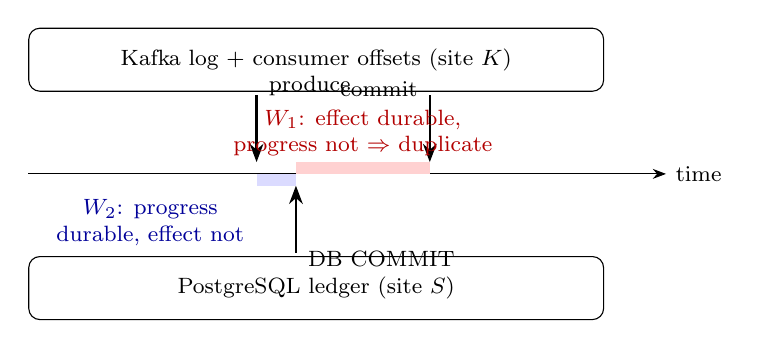
\begin{tikzpicture}[font=\footnotesize,>=Stealth,
  store/.style={draw,rounded corners,minimum height=0.8cm,align=center,inner sep=2pt},
  lab/.style={align=center}]
\draw[->] (0,0) -- (8.1,0) node[right]{time};
\node[store,anchor=west,minimum width=7.3cm] (k) at (0,1.45)
  {Kafka log + consumer offsets (site $K$)};
\node[store,anchor=west,minimum width=7.3cm] (p) at (0,-1.45)
  {PostgreSQL ledger (site $S$)};
\draw[->,thick] (2.9,1.0) -- (2.9,0.15) node[lab,above right=1pt,pos=0.2]{produce};
\draw[->,thick] (3.4,-1.0) -- (3.4,-0.15) node[lab,below right=1pt,pos=0.2]{DB COMMIT};
\draw[->,thick] (5.1,1.0) -- (5.1,0.15) node[lab,above left=1pt,pos=0.2]{commit};
\fill[red!18] (3.4,0.0) rectangle (5.1,0.15);
\fill[blue!14] (2.9,-0.15) rectangle (3.4,0.0);
\node[lab,red!70!black] at (4.25,0.52)
  {$W_1$: effect durable,\\progress not $\Rightarrow$ duplicate};
\node[lab,blue!60!black] at (1.55,-0.62) {$W_2$: progress\\durable, effect not};
\end{tikzpicture}}
\caption{The EOS boundary on a timeline. Kafka's atomic commit covers the log append
and the offset commit (top); the ledger commit is a separate single-site commit
(bottom). A crash inside either shaded interval yields exactly one durable commit:
$W_1$ duplicates under redelivery, $W_2$ loses the posting permanently. The windows are
defined by Eqs.~\eqref{eq:w1}--\eqref{eq:w2}.}
\label{fig:eos}
\end{figure}

\subsection{Assumptions, crash points, and equivalence classes}
\label{sec:model:assumptions}

Every claim in this paper is conditioned on the assumptions of
Table~\ref{tab:asm}; each is either enforced by the harness or explicitly excluded.
The fault model is crash-recovery, not Byzantine: processes die and restart, storage is
prefix-consistent, and the network may lose, delay, partition or reset connections, but
protocol checksums and retries are intact. Databases and brokers are assumed durable
once they acknowledge; clocks are used only for measurement.

\begin{table*}[t]
\centering
\small
\caption{Assumptions. Every proposition in Section~\ref{sec:formal} is stated under
A1--A13; the enforcement column names the harness mechanism that checks or excludes the
assumption.}
\label{tab:asm}
\begin{tabular}{@{}p{0.7cm}p{10.6cm}p{4.3cm}@{}}
\toprule
ID & Assumption & Enforced / excluded by \\
\midrule
A1 & Crash-recovery faults only; storage writes prefix-consistent; no Byzantine corruption. & process kills and restarts; no data mutation injected \\
A2 & Network faults are loss, delay, partition, reset; protocol checksums and retries intact. & Toxiproxy toxics only \\
A3 & PostgreSQL durable on acknowledgement (\texttt{synchronous\_commit=on}, \texttt{fsync=on}, \texttt{full\_page\_writes=on}); single instance, no replica. & pinned configuration; asserted per run \\
A4 & Kafka durable: replication factor 3, \texttt{min.insync.replicas=2}, \texttt{acks=all}, unclean leader election disabled. & pinned broker configuration \\
A5 & Transactional producer idempotence and fencing as specified; transaction timeout bounded. & pinned producer configuration \\
A6 & At most one owner per partition at a time, except inside the deliberately injected zombie window $C_7$. & pinned consumer timeouts; $C_7$ tests the exception \\
A7 & Fair recovery: killed processes restart and retry until quiescence. & runner restart policy; quiescence criteria \\
A8 & Clocks used only for latency; single host, single boot, no clock steps during a run. & clock checks around every run \\
A9 & Deterministic load; the processor is exactly-once into the source topic. & ground-truth digest and source-integrity gate \\
A10 & Faults act at declared points and every firing is attested. & fault log with one receipt per action \\
A11 & Identical configuration and tuning effort across mechanisms, except declared intrinsic components. & configuration hash audit \\
A12 & Single currency, two-leg entries, positive integer amounts; no reversals or adjustments. & event schema \\
A13 & The oracle shares no code with the pipeline and reads ground truth created before the effect. & independent process and language \\
\bottomrule
\end{tabular}
\end{table*}

Table~\ref{tab:crashpoints} enumerates the crash points of the mechanism skeleton: the
places where a process may die, a message may be lost or duplicated, or two durable
transitions may become visible in an order different from the program order. The list
is exhaustive for the skeleton of Section~\ref{sec:mechanisms} (read, effect, progress,
publish). Points that are outcome-equivalent for the invariants are grouped into the
classes $K_1$--$K_7$ of Table~\ref{tab:kclasses}; classes are used as the cells of the
structural experiment, and the equivalence arguments are the proofs that a class may be
represented by one member.

\begin{table*}[t]
\centering
\small
\caption{Crash-point model. ``Durable at the point'' is the state that survives the
crash; the last column names the window of Eqs.~\eqref{eq:w1}--\eqref{eq:w2}.}
\label{tab:crashpoints}
\begin{tabular}{@{}p{0.6cm}p{6.3cm}p{4.2cm}p{4.6cm}@{}}
\toprule
ID & Crash point & Durable at the point & Window / consequence \\
\midrule
$C_1$ & after fetch, before any durable operation & nothing of the batch & none; replay \\
$C_2$ & inside the effect transaction, before COMMIT is sent & nothing (transaction aborts) & none; replay \\
$C_3$ & after effect COMMIT is sent, before its acknowledgement & effect unknown; progress behind & $W_1$, conditional on the outcome \\
$C_4$ & after effect durable, before progress durable & effect durable; progress behind & $W_1$ (duplicate under redelivery) \\
$C_5$ & after progress durable, before effect durable & progress durable; effect absent & $W_2$ (posting lost permanently) \\
$C_6$ & duplicate delivery without a crash (rebalance reassignment, offset rewind) & unchanged & $W_1$ replay \\
$C_7$ & zombie writer: paused owner resumes after reassignment and writes & the new owner's effect & duplicate write; fencing or dedup needed \\
$C_8$ & publish window: publish sent/lost without a durable publication mark & ledger durable; publication not & publication integrity only \\
$C_9$ & sink-link loss during effect commit (partition, reset) & effect unknown; progress behind & $W_1$, conditional \\
$C_{10}$ & Kafka-side disruption during progress commit (broker kill, coordinator failover, abort) & effect durable; progress not & $W_1$; aborted transaction also discards stream records \\
$C_{11}$ & acknowledgement before durability at either store & unknown & both windows; excluded by A3/A4 \\
$C_{12}$ & partial-batch durability (per-record autocommit) & part of the batch & $W_1$ partial; unreachable with one transaction per batch \\
\bottomrule
\end{tabular}
\end{table*}

\begin{table}[t]
\centering
\small
\caption{Equivalence classes of crash points for the invariants I1--I4. Two points are
equivalent when, for every admissible schedule at one, a schedule exists at the other
with the same durable projection at recovery.}
\label{tab:kclasses}
\begin{tabular}{@{}p{0.7cm}p{1.8cm}p{4.7cm}@{}}
\toprule
Class & Members & Equivalence reason \\
\midrule
$K_1$ & $C_1,C_2$ & no durable trace; identical replay \\
$K_2$ & $C_3,C_9$ & effect possibly durable, progress behind; same unknown-outcome recovery \\
$K_3$ & $C_4,C_{10}$ & effect durable, progress behind; $C_{10}$ additionally aborts stream records \\
$K_4$ & $C_5$ & progress durable, effect absent \\
$K_5$ & $C_6$ & duplicate delivery with progress state ``not yet processed'' \\
$K_6$ & $C_7$ & two concurrent writers of one partition \\
$K_7$ & $C_8$ & ledger and progress durable; publication durability only \\
\bottomrule
\end{tabular}
\end{table}


% ============================================================================
% sections/mechanisms.tex -- Section 4: Mechanisms (compressed)
% ============================================================================

\section{Mechanisms}
\label{sec:mechanisms}

All mechanisms implement one skeleton. The service polls a batch $B$ of source records and
performs up to three durable duties: \emph{D-effect} appends the batch's postings to the
ledger sink; \emph{D-progress} makes the batch's consumption progress durable;
\emph{D-publish} appends derived entry records to the publication stream. A mechanism is
defined by (i) whether D-effect and D-progress are one atomic commit, (ii) the ordering of
the two when they are not, (iii) whether the effect is idempotent under the business key, and
(iv) how D-publish is made recoverable. The six mechanisms and three combinations below are
the points of that design space that practitioners deploy; the naive and Kafka-internal
variants are controls. The experiment measures both the correctness consequence and the cost,
which is what RQ2 asks for.

Throughout, $B$ denotes a poll batch, $\Pi(e)$ the expected posting pair of event $e$,
$\mathit{insert\_plain}$ a plain \texttt{INSERT}, and $\mathit{insert\_idem}$ an insert that is
a no-op when $(\mathit{event\_id},\mathit{leg\_no})$ already exists
\cite{pg-onconflict}. Every mechanism uses one database transaction per poll batch; the
per-record-autocommit variant is analysed as crash point $C_{12}$ but not deployed.

\subsection{The mechanisms}
\label{sec:mechanisms:defs}

\paragraph{M0 --- naive at-least-once (negative control).}
M0 commits the postings with a plain insert, publishes on a best-effort basis, and only then
commits offsets; it is the mechanism a team writes first: correct in the absence of faults,
and the reference point against which the others must improve. Its ledgers have no
de-duplication constraint, so any redelivery between the effect commit and the offset commit
duplicates postings.

\paragraph{M1 --- Kafka exactly-once, two sink variants.}
M1 (Algorithm~\ref{alg:m1}) performs the Kafka-internal appends inside a transaction
\cite{kip98,kip447,kafka-design}. In \emph{M1-kafka} the ledger \emph{is} the publication
stream: entries appended inside the transaction are the ledger, so durable effects and offsets
are one atomic Kafka commit and no external store is involved --- the positive control of the
paper. In \emph{M1x} the same transaction wraps the stream appends, but the ledger rows are
written by a separate, non-atomic database commit between the produce step and the transaction
commit. This is the deployment the paper is about: practitioners keep Kafka's exactly-once for the
internal stream and assume it covers the external write. It is not a straw man --- the
transaction is the documented way to obtain internal exactly-once, and the external write is
typically added as an ordinary database call in the same method: precisely the non-atomic
ordering of Algorithm~\ref{alg:m1}.

\begin{algorithm}[t]
\footnotesize
\begin{algorithmic}[1]
\State \textbf{on assignment} $p$: seek to committed offset
\Loop
  \State $B \gets \Call{Poll}{ }$
  \State \Call{TxnBegin}{ }
  \ForAll{$r \in B$}
    \State \Call{TxnSend}{stream, entry($r$)} \Comment{inside $T$}
  \EndFor
  \If{DB sink (M1x)}
    \State \Call{DbBegin}{}; insert postings of $B$; \Call{DbCommit}{} \Comment{outside $T$}
  \EndIf
  \State \Call{SendOffsetsToTxn}{$B$} \Comment{inside $T$}
  \State \Call{TxnCommit}{ } \Comment{stream and offsets atomic}
\EndLoop
\end{algorithmic}
\caption{M1 family: Kafka transaction (M1-kafka and M1x)}
\label{alg:m1}
\end{algorithm}

\paragraph{M2 --- transactional outbox with inbox de-duplication.}
M2 (Algorithm~\ref{alg:m2}) makes the database transaction the atomic unit. Inside it, the
mechanism claims each event in an \emph{inbox} table whose primary key is
$\mathit{event\_id}$, inserts the postings only for successfully claimed events, and writes an
\emph{outbox} row describing the publication intent. The database commit is therefore
simultaneously the effect, the de-duplication record and the publication intent. Offsets are
committed afterwards; redelivery finds the claim and becomes a no-op. A relay thread reads
unmarked outbox rows and publishes them, marking each row after the broker acknowledgement.
This is the outbox pattern as documented for microservice integration
\cite{debezium-outbox,laigner2021,micro2026}; it buys recoverable publication at the cost of
two extra durable writes per event and a background thread. (Sagas
\cite{sagas1987,saga2019} compensate rather than make commits atomic and are outside the
pipeline model studied here.)

\begin{algorithm}[t]
\footnotesize
\begin{algorithmic}[1]
\State \textbf{consumer loop}
\Loop
  \State $B \gets \Call{Poll}{ }$
  \State \Call{DbBegin}{ }
  \ForAll{$r \in B$}
    \State \Call{ClaimInbox}{r} $\rightarrow \mathit{claimed}$ \Comment{claim if absent}
    \If{$\mathit{claimed}$}
      \State \Call{insert\_plain}{$\Pi(\mathrm{parse}(r))$}
      \State \Call{AppendOutbox}{$r$}
    \EndIf
  \EndFor
  \State \Call{DbCommit}{ } \Comment{effect, inbox and outbox atomic}
  \State \Call{CommitOffsets}{$B$}
\EndLoop
\Statex
\State \textbf{relay thread}
\Loop
  \State $R \gets \Call{UnpublishedOutbox}{ }$
  \ForAll{$o \in R$}
    \State \Call{Publish}{$o$}; on ack \Call{MarkPublished}{$o$}
  \EndFor
\EndLoop
\end{algorithmic}
\caption{M2: transactional outbox with inbox claim and relay}
\label{alg:m2}
\end{algorithm}

\paragraph{M3 --- idempotency key with a unique index.}
M3 adds a unique index on the pair (event identifier, leg number) and inserts every leg with
a conflict-ignoring insert (\texttt{ON CONFLICT DO NOTHING}); a redelivery is absorbed by the
index, so the effect becomes idempotent without any additional table, and offsets are committed
after the database commit. The mechanism is the cheapest de-duplication known in practice ---
idempotency keys are the standard recipe for safe retries in public
APIs~\cite{stripe-idempotency} --- but, as Section~\ref{sec:formal} shows, it
protects against duplicates only: a posting never written is not restored by a unique index.

\paragraph{M4 --- offsets in the same transaction as the postings.}
M4 (Algorithm~\ref{alg:m4}) removes Kafka from the recovery path for correctness: the database
transaction contains both the postings and the progress row $\mathit{next\_offset}$ per
partition. On assignment --- including after every rebalance \cite{kip429} --- the consumer
seeks to the stored offset, not the Kafka-committed one. Kafka offsets may still be committed
for observability, but they are never consulted for recovery. No de-duplication index is
needed for the crash points that keep progress behind the effect, because a durable effect
implies a durable progress row; the open case is a second writer of the same partition
($C_7$). Seeking on assignment makes M4 recoverable: the group protocol can move a partition at any
moment \cite{kip429}, and a mechanism whose recovery point is a Kafka offset cannot know
whether the transaction that wrote the last batch also advanced it. M4 makes the database
transaction the only recovery point, and the monotone guard prevents a late writer from moving
the offset backwards.

\begin{algorithm}[t]
\footnotesize
\begin{algorithmic}[1]
\State \textbf{on assignment} $p$: $o \gets$ \Call{StoredOffset}{p}; seek $p$ to $o$
\Loop
  \State $B \gets \Call{Poll}{ }$
  \State \Call{DbBegin}{ }
  \ForAll{$r \in B$}
    \State \Call{insert\_plain}{$\Pi(\mathrm{parse}(r))$}
  \EndFor
  \ForAll{partitions $p$ in $B$}
    \State \Call{AdvanceProgress}{$p,\ \mathrm{end}(B,p)$} \Comment{monotone guard}
  \EndFor
  \State \Call{DbCommit}{ } \Comment{effect and progress atomic}
  \State \Call{Publish}{$B$}
\EndLoop
\end{algorithmic}
\caption{M4: offsets stored in the posting transaction}
\label{alg:m4}
\end{algorithm}

\paragraph{Combinations.}
Three combinations complete the design space for RQ3. \emph{M2+M3} replaces M2's inbox claim
by the posting unique index: the outbox is still written, but the de-duplication record is the
posting itself. \emph{M4+M3} adds the unique index to M4, closing the concurrent-writer
exposure. \emph{M1x+M3} adds the unique index to M1x's external write, keeping Kafka-internal
exactly-once for the publication stream. Other combinations are dominated in the model: M2+M4
closes no exposure that M4 does not already close, M0+M3 is M3, and three-way combinations add
cost without closing an additional exposure class.

\subsection{Distinctness, ordering, and failure handling}
\label{sec:mechanisms:compare}

The mechanisms are genuinely distinct: no two configurations share the same combination of
atomicity, idempotence, publication path and recovery source of truth. The comparison is the
bridge to Section~\ref{sec:formal}: each configuration closes a different subset of the two
windows of Eqs.~\eqref{eq:w1}--\eqref{eq:w2}.




The design space is summarised by four properties: \emph{atomicity} (effect and progress commit
together), \emph{idempotence} (the effect is deduplicated on the pair event identifier/leg
number), \emph{publication path} (inline, or inside the Kafka transaction, or through an outbox
relay) and \emph{recovery source} (Kafka offsets, the Kafka transaction, or a database progress
row). M0 and M1x are neither atomic nor idempotent; M1-kafka is atomic at the Kafka site with an
implicit transaction-level dedup; M2 is atomic at the database with an inbox primary key and an
outbox relay; M3 is idempotent through a posting unique index; M4 is atomic at the database
through a progress row. The combinations add the missing property to their base mechanism:
M2+M3 replaces the inbox key by the posting index, M4+M3 adds the index against the concurrent
writer, and M1x+M3 adds it to the external write while keeping Kafka-internal exactly-once for
the publication stream.

\paragraph{Commit ordering.}
For mechanisms that do not commit both duties at one site, the program order of
$\mathrm{Commit}_{S}$ (effect) and $\mathrm{Commit}_{K}$ (progress) selects which window of
Lemma~\ref{lem:windows} stays open. All mechanisms are deployed in \emph{strict} order ---
effect before progress --- so $W_2$ is out of reach and $W_1$ is the exposure that
de-duplication must close. Because H3 concerns the loss window, every mechanism is additionally
instrumented with an \emph{early} variant that commits progress before the effect; early is a
probe, not a candidate design, and exists to make $W_2$ observable under a deterministic crash
point ($C_5$, class $K_4$). The probe uses the same code path with a single ordering flag, so it
cannot be dismissed as a code mutation; the bounded model of Section~\ref{sec:formal} reproduces
both orderings.

\paragraph{Failure handling.}
The retry policies form part of each mechanism's definition: they determine whether an unknown
commit outcome is re-established by re-execution or by checking the de-duplication state. After a
definite failure every mechanism retries (M0/M1x up to three times with backoff, then replay);
after an unknown outcome only a mechanism that can re-establish the outcome from its
de-duplication state or stored progress may retry safely --- M2 and M3 do so through the inbox
and the unique index, M4 re-reads stored progress and skips if it advanced, while M0/M1x must
replay without a write retry. Kafka-offset or transaction-commit failures are retried by
M0/M1x/M2/M3 and are best effort for M4, which never uses Kafka offsets for recovery; a fenced
M1 transaction aborts and restarts the instance. Fixing the policy as part of the mechanism
definition prevents a comparison in which one mechanism benefits from a more optimistic retry
rule than another.

\paragraph{Fairness contract.}
All mechanisms share the same client, broker, database and JVM settings; the configuration is
hashed per run and an audit rejects any run whose shared part differs (Section~\ref{sec:method}).
Only mechanism-intrinsic components may differ: M1's transactional producer, M2's inbox/outbox
tables and relay, the de-duplicating index, and M4's progress table. No mechanism receives
per-mechanism tuning; a configuration change found during the pilot is applied wherever it
applies and recorded as a deviation. This contract makes the performance comparison a comparison
of mechanisms, not of tuning effort.


% ============================================================================
% sections/formal.tex -- Section 5: Invariant Preservation (compressed; all
% propositions, lemmas and traces retained; the counterexample-trace table and
% closure table are now prose)
% ============================================================================

\section{Invariant Preservation}
\label{sec:formal}

This section states the preservation results the experiment is designed to test. The
propositions are falsifiable predictions: each names the invariant, the window or crash point
it concerns, and the measurement that can refute it. Proof sketches are given for the closure
results and concrete counterexample traces for the violations. A bounded TLA+
\cite{lamport1994} model complements the argument; it was machine-checked with TLC at the
bounds of Section~\ref{sec:formal:tlc} and is a bounded witness of the crash-point semantics,
not an unbounded proof.

\subsection{Closure conditions}
\label{sec:formal:closure}

Lemma~\ref{lem:windows} leaves two ways to close the windows
Eqs.~\eqref{eq:w1}--\eqref{eq:w2}: make the effect idempotent, or make effect and progress one
atomic commit. Lemma~\ref{lem:closure} records which property closes which window; a two-site
2PC protocol closes both, but the analysed pipeline does not use one.

\begin{lemma}[Closure]
\label{lem:closure}
A mechanism preserves I3 against a schedule in $W_1$ if and only if its effect is idempotent
under the business key $(\mathit{event\_id},\mathit{leg\_no})$ or its effect and progress are
one atomic commit. A mechanism preserves I4 against a schedule in $W_2$ if and only if its
effect and progress are one atomic commit; de-duplication is irrelevant to $W_2$.
\end{lemma}

\begin{proofsketch}
($W_1$, $\Leftarrow$) An idempotent effect makes re-execution a no-op; atomic
effect+progress means a durable effect implies durable progress, so no redelivery occurs.
\end{proofsketch}

Lemma~\ref{lem:closure} classifies every mechanism: M0 and M1x fail $W_1$; M3 fails $W_2$ under
the early probe; M4 and M2 have atomicity and fail neither, except M4's concurrent-writer
exposure ($C_7$); the combinations add the missing property. This is the model's answer to RQ1;
Table~\ref{tab:crashverdicts} lists the predictions the measurements can refute.

\subsection{Propositions}
\label{sec:formal:props}

\begin{proposition}[EOS boundary]
\label{prop:p1}
Kafka's atomic commit covers exactly the transitions of Eq.~\eqref{eq:eos}; for every mechanism
except M1-kafka the ledger commit is outside it, so under $W_1$ the internal publication stream
and the external ledger can both be ``correct'' on their own terms while diverging from each
other.
\end{proposition}
\begin{proofsketch}
By construction of the boundary: the transaction includes Kafka appends and offsets, and the
database commit is a separate site (Corollary~\ref{cor:eosgap}).
\end{proofsketch}

\begin{proposition}[$W_1$ closure]
\label{prop:p2}
Under strict ordering and crash-recovery faults, a mechanism preserves I3 in every schedule of
$W_1$ if and only if it is idempotent under the business key or commits effect and progress
atomically.
\end{proposition}
\begin{proofsketch}
Lemma~\ref{lem:closure} applied to the $W_1$ schedules; the counterexample is trace X1 and the
positive cases are trace X2 (index) and X5 (atomicity).
\end{proofsketch}

\begin{proposition}[$W_2$ closure]
\label{prop:p3}
A mechanism preserves I4 against the early-ordering probe if and only if its effect and
progress are one atomic commit; de-duplication cannot restore a posting that was never written.
\end{proposition}
\begin{proofsketch}
Trace X3: progress is durable, the effect is absent, and the batch is never redelivered, so the
posting is missing irrespective of any unique index.
\end{proofsketch}

\begin{proposition}[M0 negative control]
\label{prop:p4}
M0 yields duplicates (I3 violations) under the deterministic $W_1$ injection and under duplicate
redelivery, because it has neither de-duplication nor atomic progress.
\end{proposition}
\begin{proofsketch}
Lemma~\ref{lem:closure}, failure direction.
\end{proofsketch}

\begin{proposition}[M1-kafka positive control]
\label{prop:p5}
M1-kafka preserves I1--I4 in every executed cell: both duties are inside one Kafka transaction
\cite{kip98}, and the publication stream is its own ledger.
\end{proposition}
\begin{proofsketch}
A replay of an uncommitted transaction produces no durable record, and a committed transaction
carries its offsets atomically; producer fencing excludes a zombie.
\end{proofsketch}

\begin{proposition}[M1x fails where the gap opens]
\label{prop:p6}
M1x yields duplicates (I3) in the $W_1$ crash classes and the corresponding fault conditions,
while its publication stream remains exactly-once; it has no $W_2$ exposure under strict
ordering.
\end{proposition}
\begin{proofsketch}
The ledger rows are committed outside the transaction, while the stream records and the offsets
are inside it; a crash between the database commit and the transaction commit (trace X4)
duplicates the ledger and discards the stream record of the aborted transaction.
\end{proofsketch}

\begin{proposition}[M2 sufficiency]
\label{prop:p7}
M2 preserves I1--I4 in all executed cells: the inbox claim makes redelivery a no-op, the
database transaction makes the effect atomic, and the outbox makes publication recoverable.
\end{proposition}
\begin{proofsketch}
Each $W_1$ schedule is absorbed by the claim (trace X2 with a table instead of an index); $W_2$
is unreachable under strict ordering; the relay window concerns only publication (trace X7).
\end{proofsketch}

\begin{proposition}[M3: duplicates closed, losses open]
\label{prop:p8}
M3 preserves I1--I4 in the $W_1$ crash classes and yields no duplicate in any modelled condition,
but loses postings under the early-ordering probe.
\end{proposition}
\begin{proofsketch}
The unique index absorbs every replay ($W_1$, trace X2).
\end{proofsketch}

\begin{proposition}[M4: atomicity without de-duplication]
\label{prop:p9}
M4 preserves I1--I4 in the $W_1$ and $W_2$ crash classes because effect and progress are one
database transaction, but it is exposed to a concurrent writer ($C_7$).
\end{proposition}
\begin{proofsketch}
A durable transaction advances the stored offset atomically, so a crash can only leave both or
neither durable ($W_1$/$W_2$ unreachable, trace X5).
\end{proofsketch}

\begin{proposition}[Combinations]
\label{prop:p10}
M2+M3, M4+M3 and M1x+M3 each close exactly the exposure missing from their base mechanism and
introduce no new durable duty.
\end{proposition}
\begin{proofsketch}
Superposition of Propositions~\ref{prop:p7}--\ref{prop:p9}: the added component is a constraint
(a unique index), not a protocol step, so it cannot open a window.
\end{proofsketch}

\begin{proposition}[Balance checks are blind to duplication]
\label{prop:p11}
There are schedules in which I3 is violated while I1 holds: a duplicated balanced entry sums to
zero. Consequently a practitioner who checks only that every entry balances will not detect the
duplicates produced by the EOS gap.
\end{proposition}
\begin{proofsketch}
A second copy of a balanced entry is itself balanced; the per-entry signed sum remains zero and
the legs are structurally well-formed.
\end{proofsketch}

\begin{proposition}[No dominance]
\label{prop:p12}
Under the model no single mechanism is simultaneously complete on correctness and best on cost:
M3 is the cheapest complete ledger mechanism under strict ordering but is blind to $W_2$; M4
closes both windows without an index but is open to $C_7$ and does not preserve publication
exactly-once; M1x+M3 is required for ledger integrity plus Kafka-internal exactly-once
publication and pays the transaction cost; M2 buys recoverable publication at the highest write
cost.
\end{proposition}
\begin{proofsketch}
Lemma~\ref{lem:closure} and the design-space comparison of Section~\ref{sec:mechanisms}: each mechanism
closes a different subset, and the properties that close correctness (dedup, atomicity) are not
the properties that reduce cost.
\end{proofsketch}

\subsection{Counterexample traces}
\label{sec:formal:traces}

Four traces carry the argument; the remaining pre-registered traces (X2, duplicate absorbed
by a unique index; X7, relay window affecting only publication) are corollaries. \textbf{X1
(duplicate, $W_1$):} $b$'s effect commit returns; the process dies before the offset commit
($C_4$); on restart $b$ is redelivered and the plain insert executes again, so every posting of
$b$ occurs twice (I3 violated, I1 intact). \textbf{X3 (loss, $W_2$):} the early probe commits
progress first; the process dies before the effect is durable ($C_5$); restart resumes past $b$,
which is never redelivered, so its postings are lost (I4 violated) and an index cannot restore
them. \textbf{X4 (divergence):} $T$ produces $b$'s stream records; $b$'s database commit
returns; a broker kill aborts $T$ ($C_{10}$); the retry rewrites the ledger and commits a new
transaction, so the ledger holds two copies while the stream holds one (I3 violated, stream
exactly-once yet divergent). \textbf{X6 (zombie):} A reads $b$, is paused past the poll
interval, the partition moves to B which processes $b$, and A resumes and commits: $b$ is
written twice with nothing to stop it, so M4 needs either the index (M4+M3) or fencing.

\subsection{Predicted verdicts per crash class}
\label{sec:formal:verdicts}

Table~\ref{tab:crashverdicts} gives the model's predicted verdict for every (mechanism, crash
class) pair; the experiment measures each cell with the injector mapped to its class. Symbols:
$\mathsf{P}$ preserved; $\mathsf{V}_3$ duplicate expected; $\mathsf{V}_4$ loss expected;
$\mathsf{C}_3$ conditional on the unknown-outcome resolution; $\varnothing$ structurally
unreachable. The predictions are pre-registered; a contradicting measurement must be reported as
such.

\begin{table*}[t]
\centering
\scriptsize
\caption{Model-predicted verdicts by mechanism and crash class. $K_4$ is executed with the
early-ordering probe; the M4 and M4+M3 entries in that column are probe (degraded-variant)
results, not the canonical mechanism. $\varnothing$ marks a state that the mechanism's protocol
cannot reach (single-site atomicity or absence of a second commit).}
\label{tab:crashverdicts}
\begin{tabular}{@{}lccccccc@{}}
\toprule
Mechanism & $K_1$ & $K_2$ & $K_3$ & $K_4$ (probe) & $K_5$ & $K_6$ & $K_7$ \\
\midrule
M0        & P & C$_3$ & V$_3$ & V$_4$ & V$_3$ & V$_3$ & $\varnothing$ \\
M1-kafka  & P & P     & $\varnothing$ & $\varnothing$ & P & P & $\varnothing$ \\
M1x       & P & V$_3$ & V$_3$ & V$_4$ & V$_3$ & V$_3$ & $\varnothing$ \\
M2        & P & P     & P     & V$_4$ & P     & P     & P \\
M3        & P & P     & P     & V$_4$ & P     & P     & $\varnothing$ \\
M4        & P & P     & $\varnothing$ & V$_4^{\dagger}$ & P & V$_3$ & $\varnothing$ \\
M2+M3     & P & P     & P     & V$_4$ & P     & P     & P \\
M4+M3     & P & P     & $\varnothing$ & V$_4^{\dagger}$ & P & P & $\varnothing$ \\
M1x+M3    & P & P     & P     & V$_4$ & P     & P     & $\varnothing$ \\
\bottomrule
\end{tabular}
\par\smallskip
{\footnotesize $^{\dagger}$Probe result for the degraded early-ordering variant; the canonical
M4 and M4+M3 protocols have no separate progress commit, so $K_3$ and the canonical form of
$K_4$ are unreachable and the cell is not a pass.}
\end{table*}

\subsection{Bounded machine-checked model}
\label{sec:formal:tlc}

The crash-point semantics of Section~\ref{sec:model} were encoded in a small TLA+
\cite{lamport1994} model of per-$(\mathit{event},\mathit{leg})$ posting multiplicities, durable
progress, publication records and a crash flag. Four booleans parameterise the mechanism family:
de-duplication, atomic effect+progress, atomic publication+progress (the Kafka transaction) and
the early-ordering probe. The model is deliberately small --- three events, batches of two, one
partition --- with bounds fixed before any check.

The checked outcome is summarised here. All eight configurations matched the
expectation recorded before checking: the naive and transaction-only configurations violate the
uniqueness invariant (I3) --- a duplicate posting is reachable --- while the de-duplicating and
atomic configurations violate none, and both early-ordering probes violate completeness (I4) ---
a posting is lost while the unique index is present. The two probes are the machine-checked form
of Proposition~\ref{prop:p3}: de-duplication does not preserve completeness.


The eight checked configurations (outcome: duplicate I3, loss I4, or ``ok''): naive I3; dedup
ok; atomic ok; atomic+dedup ok; kafka-txn ok; txn-only I3; early probe I4; early+dedup I4. The
booleans are the de-duplication, atomic effect$+$progress, Kafka-transaction and early-ordering
flags; distinct-state counts vary slightly with worker scheduling (20, 18, 8, 8, 8, 39, 22, 21;
authoritative values in \texttt{tlc-summary.json}).

Three qualifications bound the claim. The model is a \emph{bounded witness} (finite state
space, not an unbounded proof), its checked scope is exactly the W1/W2 closure argument over
\code{I1Balance}, \code{I3Unique} and \code{I4CompleteWhenDone}, and it models the protocols
rather than the Java implementation, which the oracle and harness gates cover. Not modelled:
rebalancing and the zombie writer (C6/C7), append-only mutation (I2), liveness, publication
invariants, partial-batch durability (C11/C12) and multi-partition scheduling --- those rest on the
pen-and-paper argument and K6 experiments; \code{StrictProgressBound} is a tautology not counted
as evidence. Model, configurations, invocation and logs are archived with the artifact.


% ============================================================================
% sections/method.tex -- Section 6: Experimental Method
% Drafted from the P1-approved docs/prereg.md and docs/method.md (§7, §8, §9).
% DESIGN ONLY: this section contains no results and no measured numbers.
% ============================================================================

\section{Experimental Method}
\label{sec:method}

The evaluation is a staged campaign of scripted faults, verified by an independent
oracle and analysed under a pre-registered protocol. This section states the substrate,
the injectors, the oracle and its validation gates, the design of the stages, the
metrics, and the frozen statistical plan. All design constants (cell counts,
repetitions, quiescence bounds, test thresholds) were fixed before the first
measurement; the protocol and the analysis code are archived with the artifact.

\subsection{Implementation and substrate}
\label{sec:method:substrate}

The artifact is a Java~21 service (one process per consumer instance) that implements all
nine configurations behind two flags: the mechanism and the commit ordering
(\emph{strict} or \emph{early}). The load generator is a Java program that emits the
deterministic event stream and writes the ground truth; the oracle is an independent
Python program that shares no code with the service. The service emits structured phase
markers and writes its effective configuration at startup and its counters at shutdown.

The reported campaign runs on a \emph{native-process substrate}: three Kafka~3.7.2 KRaft
brokers, PostgreSQL~16.11, Toxiproxy~2.9.0 and the service, all as native Windows
processes on one host, with JDK~21.0.13.1 and Maven~3.9.9. This is an explicit deviation
from a containerised deployment: the host has no Docker, no administrator rights and no
WSL2. The substrate has three consequences that the paper carries as limitations.
First, isolation is process-level: CPU affinity, priority class, heap bounds, connection
pools and every broker/database setting are pinned and recorded per run, and the shared
configuration is hashed so that a non-intrinsic difference between mechanisms fails the
run. Second, the Kafka cluster is three processes on one operating system rather than
three machines: a broker kill is a real process death and a real leader election, but
not a machine loss. Third, container-level guarantees (cgroup limits, image digests) are
replaced by recorded process limits and SHA-256 digests of the vendored binaries, and
the periodic full-stack restart every 50 runs bounds cross-run interference. Each run
uses a fresh logical state --- new source and publication topics, a new consumer group,
and a fresh database schema --- and the identities of every process are recorded so that
an injector can target a specific one.

\subsection{Fault injection}
\label{sec:method:injection}

Two injection levels are used, because they answer different questions. \emph{Level~1}
places a fault deterministically at a named crash point of Section~\ref{sec:model}:
failpoints at fixed code locations trigger one of four actions (crash, throw, abort the
transaction, or pause) on a chosen occurrence. Level~1 is the structural experiment: a
mechanism that survives a fault placed at its worst location has absorbed it.
\emph{Level~2} applies the six scripted faults of Table~\ref{tab:faults} at random,
recorded times within the steady-state window; it measures how often a fault realises an
exposed window in a realistic timeline. Every armed injection writes two attestation
records to the fault log --- one when it fires and one when the system is restored ---
and a run whose injection did not fire is invalid, excluded and counted, with the
exclusion rate reported per cell.

\begin{table*}[t]
\centering
\small
\caption{Scripted faults (Level~2) and the crash classes they realise. Timing is either
phase-coupled (Level~1) or a seeded random offset (Level~2); every action is attested in
the fault log. F4 is split by commit direction; F6 is protocol-level duplicate
redelivery only.}
\label{tab:faults}
\begin{tabular}{@{}p{0.7cm}p{5.4cm}p{4.4cm}p{5.2cm}@{}}
\toprule
Fault & Injected condition & Mechanism manipulated & Crash classes \\
\midrule
F1 & one broker killed mid-produce (leader and transaction coordinator of the instance) & Kafka broker process, hard kill & $K_2$, $K_3$ \\
F2 & consumer instance killed during processing, forcing a rebalance & consumer process, hard kill & $K_1$--$K_3$, $K_5$ \\
F3 & produce or transaction commit times out with unknown outcome & TCP delay/timeout on the produce link & $K_2$, $K_3$ \\
F4a & effect commit durable, progress commit fails & offset-commit link cut after the effect marker & $K_3$ \\
F4b & progress commit durable, effect commit fails (early ordering probe) & ordering flag plus a database-link cut & $K_4$ \\
F5 & network partition between the service and the database & TCP blackhole/reset on the database link & $K_2$, $K_3$ \\
F6 & duplicate redelivery after a rebalance (protocol-level replay) & consumers stopped, resume point rewound, consumers resumed & $K_5$ \\
\bottomrule
\end{tabular}
\end{table*}

\subsection{Independent oracle and ground truth}
\label{sec:method:oracle}

Correctness is measured against ground truth created \emph{before} the effect: the
generator derives the whole event stream from the repetition seed, writes one canonical
line per expected posting to a ground-truth file, computes its SHA-256, and fsyncs both
before producing the first record. After the run, the oracle (i) regenerates the expected
posting set from the seed with its own implementation, (ii) checks that the regenerated
digest equals the pre-send digest, (iii) dumps the source topic and checks that it is
contiguous and exactly matches the produced manifest, and (iv) compares the sink against
the expected multiset. Only when the first three checks pass is $\Omega$ well defined
and the run eligible for analysis. The oracle reads the sink through a read-only role
and computes the invariants I1--I4 of Table~\ref{tab:invariants} and the verdict of
Eq.~\eqref{eq:consistency} directly from the dumps.

Two properties of the oracle protect the conclusions. The first is independence: it is a
separate program in a different language, with no shared code, and ground truth exists
before the pipeline runs. The second is mutation testing: before any measurement, the
checker is attacked with seeded synthetic defects --- a dropped posting, a duplicated
posting, a flipped leg sign, an updated row, and a spurious posting, at least one hundred
mutations per class --- and it must detect one hundred percent of them, attributed to the
correct invariant. A checker that misses a defect class invalidates the campaign rather
than a mechanism. The approach follows the systematic-testing tradition of crash
consistency \cite{crashmonkey2019} and isolation-anomaly checking \cite{elle2020}: the
verifier is an independent executable model of the property, not an assertion inside the
system under test.

\textbf{Quiescence.} A run is observed only in a quiescent state: consumer lag is zero
for all source partitions, no new sink row has appeared for ten seconds, no application
transaction is active, and the retry drain interval has elapsed. If quiescence is not
reached within a pre-registered bound of 300~s, the run is \emph{censored}: it counts as
a violating run (or as a quiescence failure if the application is still active) rather
than being dropped. The final observation is a single repeatable-read snapshot
\cite{pg-isolation}.

\subsection{Harness-validation gates}
\label{sec:method:gates}

No measurement is analysed until the gates of Table~\ref{tab:gates} pass. The gates are
deliberately adversarial: the negative control must fail, the positive controls must pass,
and the oracle must catch synthetic defects before it is trusted to judge the pipeline.
The gate that most often reveals a design error is the negative control: M0 is expected
to produce duplicates under the deterministic $W_1$ injection, so a clean M0 means the
injector or the oracle is broken, not that naive at-least-once is safe.

\begin{table*}[t]
\centering
\small
\caption{Harness-validation gates. G1--G8 must pass on pilot data before any experimental
run is analysed; failures halt the campaign.}
\label{tab:gates}
\begin{tabular}{@{}p{0.7cm}p{8.3cm}p{6.4cm}@{}}
\toprule
Gate & Requirement & Failure action \\
\midrule
G1 & negative control: M0 shows duplicates under the deterministic $W_1$ injection, with attestation & halt; harness broken \\
G2 & positive controls: M1-kafka and M4+M3 show no violation in fault-free runs & halt \\
G3 & checker mutation testing: 100\,\% detection of drop, duplicate, sign flip, update, spurious row ($\geq 100$ mutations per class) & fix checker; repeat \\
G4 & injector attestation: one fired and one restored record per armed injection; exclusion rate computed from receipts only & exclude and count; flag cell if $>20\,\%$ \\
G5 & ground-truth independence: generator digest equals oracle digest; source-integrity gate passes & invalidate runs; fix derivation \\
G6 & configuration equality: shared configuration hash identical across mechanisms; only declared intrinsic keys differ & halt; unfair comparison \\
G7 & load-generator capability: sustained $\geq 3\times$ the fastest measured mechanism throughput; doubling the quiet period does not change any count & resize generator; recalibrate quiescence \\
G8 & clock and host sanity: single boot, no clock step, free disk above the floor, affinity and priority as pinned & flag or rerun \\
\bottomrule
\end{tabular}
\end{table*}

\subsection{Design, metrics, and statistics}
\label{sec:method:design}

The campaign is staged so that the structural questions are answered cheaply and
deterministically before the frequency and performance questions are measured under load
(Table~\ref{tab:stages}). Stage~A runs every reachable crash class through every
mechanism with deterministic Level-1 injections at small load; its cells are the 52
reachable (mechanism, crash-class) pairs of Table~\ref{tab:crashverdicts} plus one
control cell per mechanism. Stage~B applies the six scripted faults at random times to
all mechanisms at the canonical operating point and adds the sensitivity blocks. Stage~C
measures performance in the fault-free case; Stage~D reuses Stage~B runs for performance
under faults and for time-to-consistent-state. The campaign was pre-registered with an
unattended wall-clock budget of 8--24 hours; if the pilot projection exceeds the budget,
a fixed cut ladder is applied in order --- the large-load block first, then the partition
sensitivity block, then repetitions down to the pre-registered floor for correctness
cells; control cells are never cut.

\begin{table*}[t]
\centering
\small
\caption{Staged design. Repetitions $N$ apply per cell; ``cells'' counts executed
(mechanism, condition) pairs, with structurally unreachable cells recorded as not
applicable rather than as passes. The total is 7{,}866 matrix runs plus 20 validation
runs. No number in this table is a measurement.}
\label{tab:stages}
\begin{tabular}{@{}p{0.7cm}p{4.6cm}p{5.0cm}p{1.4cm}p{1.5cm}@{}}
\toprule
Stage & Purpose & Design & $N$ & Runs \\
\midrule
P & calibrate per-run cost, validate oracle and injectors, measure capacity for the target-rate rule & 9 mechanisms $\times$ 8 conditions $\times$ 1k events, 3 partitions & 3 & 216 \\
A & structural correctness under deterministic crash points & 52 crash-class cells + 9 control cells $\times$ 1k events, 3 partitions & 30 & 1{,}830 \\
B & correctness under stochastic faults at realistic load, plus sensitivity & 67 fault cells $\times$ 100k events, 6 partitions; sensitivity blocks at 10k events & 30 / 10 & 4{,}020 \\
C & performance, fault-free & 9 mechanisms $\times$ 2 loads $\times$ 3 partition counts; large-load and capacity blocks & 30 / 10 & 1{,}800 \\
D & performance under faults and time-to-consistent-state & reuse of Stage~B runs & --- & 0 \\
\bottomrule
\end{tabular}
\end{table*}

\paragraph{Metrics.}
Correctness is measured per run by the counts of duplicate postings ($\mathrm{I3}$),
lost postings ($\mathrm{I4}$), imbalanced entries ($\mathrm{I1}$) and mutated postings
($\mathrm{I2}$), and by the binary outcome \emph{violating run} --- any of the four
counts positive. Performance is measured in two modes. In the \emph{fixed-rate} mode the
generator offers events at a target rate independent of the service, so latency is not
corrupted by coordinated omission; in the \emph{saturation} mode the offered rate is far
above capacity and the outcome is achieved throughput. End-to-end latency of an event is
the interval from its scheduled emission to the observation that the effect commit for
its batch returned; per-run percentiles p50, p90, p99 and p99.9 are recorded with
HdrHistogram \cite{hdrhistogram} at a pre-registered precision and range. The first
$\max(2000,\,10\,\%)$ events of a run are discarded from performance statistics as
warm-up and retained for correctness. Throughput is committed events over the
steady-state window. Time-to-consistent-state is the interval from the end of load to the
first quiescent sample, and is reported with the censoring rate. Measurement practice
follows the benchmarking literature: fixed machine state and identical configuration for
all mechanisms, median and IQR rather than single observations, tail percentiles rather
than means \cite{dean2013}, awareness that small configuration differences can reverse
conclusions \cite{mytkowicz2009,raasveldt2018}, explicit reporting of the measurement
setup \cite{hoefler2015}, and statistically rigorous treatment of JVM effects
\cite{georges2007}. The design adopts the benchmarking discipline advocated for stream
processing engines \cite{theodolite2021}.

\paragraph{Frozen statistics.}
The analysis plan was frozen, together with the analysis code, before the first
experimental run; anything not in the plan is labelled exploratory. For correctness,
each cell reports the proportion of violating runs with an exact
Clopper--Pearson 95\,\% confidence interval \cite{brown2001,jsta2014}; when no violation
is observed, the rule-of-three bound is reported as a conservative summary
\cite{rule3} and the text states explicitly that the bound does not prove absence.
Mechanisms are compared with McNemar's exact test on paired runs --- the same repetition
seeds are used for every mechanism within a cell, so the comparison is paired
\cite{mcnemar1947} --- with Fisher's exact test as an unpaired sensitivity analysis, and
Holm's correction within pre-declared families \cite{holland1987}. For performance, each
cell reports median and IQR with a bootstrap 95\,\% confidence interval (10{,}000
resamples, recorded seed) \cite{efron1979}; mechanisms are compared with the Friedman
test over blocks of load and partition count, Nemenyi post-hoc analysis, and Cliff's
delta with pre-registered magnitude thresholds (negligible below 0.147, small below 0.33,
medium below 0.474) \cite{demsar2006,cliff1993}. The level is $\alpha=0.05$ throughout,
unadjusted and adjusted $p$-values are both reported, all $N$ and exclusion rates are
reported per cell, and power statements accompany zero-event claims. Statistical
practice follows the guidance for randomised and benchmark comparisons in software
engineering \cite{arcuri2011,arcuri2012}, and the raw data, seeds and frozen scripts
are released so that every table can be regenerated \cite{collberg2016}.


% Section 7 — Results. DATA STATUS: the confirmatory campaign is being executed on the
% approved Linux/container host; this section fixes the reporting structure and is filled
% exclusively from frozen run records by tools/analyze.py and tools/make-figures.py.
% No value in this section is typed by hand; every float is marked PENDING until generated.
\section{Results}
\label{sec:results}

\textbf{Data status.} The confirmatory campaign is executed from the frozen matrix and analysis
plan of Section~\ref{sec:method}; at preparation time it is in progress on the approved
Linux/container host, and the Windows feasibility run stopped before any confirmatory cell. Every
table and figure here is generated by the frozen pipeline from accepted run records; none is typed
by hand, and each is marked \emph{PENDING} until the pipeline emits its content.

\subsection{Campaign integrity and harness validation}
\label{sec:res-integrity}

Before any confirmatory run is analysed, the eight harness gates of Section~\ref{sec:method}
must pass: the negative control must duplicate, the positive controls must not, the checker must
detect every synthetic mutation, every armed injector must leave a complete fired/restored
receipt pair, the ground-truth digests must agree between generator and oracle, and the shared
configuration hash must be identical across mechanisms. Table~\ref{tab:validation} records the
gate evidence and the per-cell exclusion of runs whose fault did not fire; no other exclusion is
permitted.

\IfFileExists{results/analysis/tables/t1-validation.tex}{\input{results/analysis/tables/t1-validation.tex}}{%
\begin{center}
\footnotesize
\fbox{\parbox{0.92\linewidth}{\centering\textbf{Table PENDING.} Gates G1--G8: evidence and
per-cell exclusion rates, generated from frozen validation records.}}
\captionof{table}{Harness-validation evidence and exclusions (generated from frozen run records;
PENDING until the campaign completes).}
\label{tab:validation}
\end{center}}

\subsection{RQ1: where exactly-once ends}
\label{sec:res-rq1}

Table~\ref{tab:correctness} will report, per mechanism and fault condition, violating runs and
the one-sided Clopper--Pearson 95\,\% upper bound (rule of three for zero-event cells) under the
frozen decision rules. The pre-registered prediction is that M0 violates the one-entry-per-event
invariant (I3) whenever the duplicate window is reachable, M1-kafka violates no ledger invariant,
and M1x violates in the classes the crash-point model maps to the external commit
(C3/C4/C9/C10); the early-ordering probe is predicted to show the loss violation (I4) for every
two-commit mechanism without database-resident progress. Table~\ref{tab:counts} decomposes
violations into duplicate, lost, imbalanced and mutated postings, and the report will state which
invariants were never observed to fail --- with exact upper bounds, never treating zero as a
proof. Figure~\ref{fig:correctness} places the outcomes against their measured cost.

\IfFileExists{results/analysis/tables/t2-correctness.tex}{\input{results/analysis/tables/t2-correctness.tex}}{%
\begin{center}
\footnotesize
\fbox{\parbox{0.92\linewidth}{\centering\textbf{Table PENDING.} Correctness by mechanism
$\times$ fault class: violating runs, $N$, one-sided 95\,\% upper bound.}}
\captionof{table}{Correctness by mechanism and fault class (generated from frozen run records;
PENDING until the campaign completes).}
\label{tab:correctness}
\end{center}}

\IfFileExists{results/analysis/tables/t3-counts.tex}{\input{results/analysis/tables/t3-counts.tex}}{%
\begin{center}
\footnotesize
\fbox{\parbox{0.92\linewidth}{\centering\textbf{Table PENDING.} Duplicate, lost, imbalanced and
mutated posting counts by mechanism.}}
\captionof{table}{Violation counts by invariant and mechanism (generated from frozen run records;
PENDING until the campaign completes).}
\label{tab:counts}
\end{center}}

\begin{center}
\IfFileExists{figures/fig-correctness.pdf}{\includegraphics[width=\linewidth]{figures/fig-correctness}}{%
\fbox{\parbox{0.92\linewidth}{\centering\textbf{Figure PENDING.} Panel~A: per-run violation
proportion by mechanism and fault class with 95\,\% intervals. Panel~B: failure classes closed
versus p99 latency overhead. Generated from frozen run records.}}}
\captionof{figure}{Correctness evidence. Panel~A: per-run ledger-invariant violation proportion by
mechanism and fault class (Clopper--Pearson 95\,\% upper bounds; structurally unreachable cells
are n/a and never counted as passes). Panel~B: failure classes whose invariant is preserved
versus p99 latency overhead relative to the naive baseline; higher and further left is better.
PENDING until the frozen analysis completes.}
\label{fig:correctness}
\end{center}

\subsection{RQ2: the cost of closing the boundary}
\label{sec:res-rq2}

Table~\ref{tab:performance} will report throughput, end-to-end latency (p50/p99/p99.9) and
time-to-consistent-state by mechanism, load and partition count, with median/IQR and bootstrap
95\,\% intervals; the pre-registered contrasts (Friedman/Nemenyi, Cliff's delta) are stated
without calling a mechanism ``fast'' or ``slow'' outside the frozen cells.
Figure~\ref{fig:performance} shows latency ECDFs (panel~A) and throughput by load and partitions
(panel~B). Closing the duplicate window has a cost: M3 maintains an index, M4 moves progress into
the posting transaction, and M2 adds an inbox claim, outbox row and relay thread.

\IfFileExists{results/analysis/tables/t4-performance.tex}{\input{results/analysis/tables/t4-performance.tex}}{%
\begin{center}
\footnotesize
\fbox{\parbox{0.92\linewidth}{\centering\textbf{Table PENDING.} Performance by mechanism
$\times$ load $\times$ partitions: throughput, p50/p99/p99.9, time-to-consistency.}}
\captionof{table}{Performance by mechanism, load and partition count (generated from frozen run
records; PENDING until the campaign completes).}
\label{tab:performance}
\end{center}}

\begin{center}
\IfFileExists{figures/fig-latency-ecdf.pdf}{\includegraphics[width=\linewidth]{figures/fig-latency-ecdf}}{%
\fbox{\parbox{0.92\linewidth}{\centering\textbf{Figure PENDING.} Panel~A: end-to-end latency
ECDFs per mechanism (fault-free runs). Panel~B: committed-event throughput by load and
partition count. Generated from frozen run records.}}}
\captionof{figure}{Performance evidence. Panel~A: end-to-end latency ECDFs per mechanism for fault-free
runs (open-loop load; warm-up excluded). Panel~B: committed-event throughput by load and
source-partition count (median across repetitions, IQR shown). PENDING until the frozen analysis
completes.}
\label{fig:performance}
\end{center}

\subsection{RQ3: minimal sufficient mechanism sets}
\label{sec:res-rq3}

Section~\ref{sec:decision} combines the frozen correctness outcomes with the measured cost
contrasts under the pre-registered derivation rule: the duplicate window is closed by M3's index
or M4's atomic progress; the loss window only by a mechanism making progress atomic with the
effect (M4, M2, M4+M3, M2+M3), never by committing progress ahead of a durable effect (which the
`early' probe violates); M1x closes neither; M1x+M3 closes duplicates while retaining
Kafka-internal exactly-once for publication. Measured cost decides among sufficient sets.

\subsection{Hypothesis verdicts}
\label{sec:res-hypotheses}

The pre-registered decision for each hypothesis is computed by the frozen decision rules of
Section~\ref{sec:method} from the run records, and a verdict is recorded exactly as the rule
computes it (confirmed, refuted, or inconclusive). Until the campaign completes every verdict
reads \emph{pending}; the values are populated by the frozen analysis pipeline, not by hand.

The five pre-registered hypotheses are: \textbf{H1} M1x violates and M1-kafka does not;
\textbf{H2} M2 is sufficient but costs throughput/latency vs.\ M3/M4; \textbf{H3} M3 alone yields
zero duplicates but losses under early ordering; \textbf{H4} M4 or M4+M3 is sufficient with lower
latency than M2; \textbf{H5} no mechanism dominates. Their verdicts are computed by the frozen
decision rules:
H1 \ResHypothesisOneVerdict; H2 \ResHypothesisTwoVerdict; H3 \ResHypothesisThreeVerdict;
H4 \ResHypothesisFourVerdict; H5 \ResHypothesisFiveVerdict. The cells read \emph{pending} until
the analysis pipeline runs, and a verdict is recorded exactly as the rule computes it (confirmed,
refuted or inconclusive).


% Section 8 — Discussion and practitioner decision table (compressed)
\section{Discussion and Decision Table}
\label{sec:decision}

\subsection{What the boundary analysis implies for practitioners}
\label{sec:dec-implications}

The boundary analysis answers the three questions as follows. For RQ1, Kafka EOS fails to
preserve ledger invariants exactly when the external write and the progress can be committed in
different orders across a crash or unknown-outcome timeout: the duplicate window (effect durable,
progress not) and the loss window (progress durable, effect not). Broker failure, consumer death,
rebalance and partition are not failures \emph{of Kafka} here; they expose the two windows. For
RQ2, mechanisms differ in \emph{which} window they close and at what cost, not in a single score.
For RQ3, the minimal sufficient set depends on the exposure the operator accepts and on whether
the external effect must be independently recoverable.

The practical consequence is that a deployment claim should name the mechanism, not the label:
``we use Kafka exactly-once'' says nothing about the external store, whereas ``we commit the
ledger and the progress in one database transaction'' (M4) says everything about both windows,
with a residual zombie-writer exposure that an idempotency index closes (M4+M3). Operators who
cannot move progress into the database can use an atomic ledger transaction plus a deduplication
claim (M2), at the cost of an inbox/outbox write and a relay; operators who must keep the Kafka
transaction for the publication stream can add an index to the external write (M1x+M3), which
closes duplicates but not losses.

\subsection{Practitioner decision table}
\label{sec:dec-table}

The decision summary below maps a failure exposure to the minimal mechanism set that closes it, the
model's argument for that coverage, and what the executed reduced programme observed. It is
derived from the formal results of Section~\ref{sec:formal} and the descriptive evidence of
Section~\ref{sec:results}; because the reduced programme has $N=3$ per cell and no measured
fixed-rate/saturation performance block, the cost is stated qualitatively rather than as a
measured contrast. Every entry is either a model-derived claim or an observation traceable to
\texttt{results/analysis-reduced/}; none is set by hand.

\paragraph{Decision summary.} (i) $W_1$ duplicate exposure: the minimal sufficient mechanism is
an idempotency key (M3) or a transactional outbox (M2); M4 includes it atomically. Reduced
evidence: K3 duplicated only in the unguarded M0/M1x, while M1x+M3, M2, M2+M3 and M3 were clean.
(ii) $W_2$ lost-effect exposure: no mechanism in the suite closes the early-ordering probe;
prevention requires effect-before-progress durability plus reconciliation. Reduced evidence: the
K4 probe lost postings in all 24 of 24 runs (272--494 per cell), across every exposed mechanism.
(iii) $K_1$/$K_2$ (nothing durable, or unknown outcome): plain at-least-once suffices when the
effect is retried and either idempotent or absent; both classes were clean in 44 runs, including
M0. (iv) Scale (100k+, saturation): depends on load and is not measured here; the reduced
programme reports committed-event throughput only, with no ranking claim, and the pre-registered
Stage~B/C remain future work on the intended host.

A caution accompanies the table: zero-observed cells carry a rule-of-three upper bound, evidence
of practical adequacy at the tested sample size, not a proof of impossibility. The word
``certified'' is reserved, per the pre-registered language rule, for cells where the formal model
proves the invariant under the mechanism's assumptions \emph{and} the deterministic adversarial
runs are clean; a purely empirical zero is reported as ``no violation observed in $N$ runs''.

\subsection{When the extra machinery is not worth it}
\label{sec:dec-negative}

Not every pipeline needs atomic progress. If duplicates can be corrected upstream before they
affect balances, or the sink is idempotent by construction, an at-least-once pipeline with an
idempotency index may suffice and be cheaper. The decision table therefore begins with the
exposure question --- which window is reachable, what a duplicate or lost posting costs, and
whether the external effect is independently recoverable --- before the measured cost column
matters.

\subsection{Relation to prior work}
\label{sec:dec-prior}

The model is consistent with the vendor's statement of the boundary~\cite{kafka-design} and
KIP-98's producer-scoped guarantee~\cite{kip98}, but makes structural what those documents state
qualitatively: both windows are reachable under ordinary fault schedules. It extends
stream-processing fault-tolerance results~\cite{flink2017,millwheel2013} by showing that
snapshot-style reasoning protects internal state but not an external database, gives the
outbox/idempotency patterns~\cite{debezium-outbox,stripe-idempotency} a correctness--cost profile
in the ledger setting, and supplies the consistency contract missing from microservice
surveys~\cite{laigner2021,micro2026}.

\subsection{Reusability of the method}
\label{sec:dec-reuse}

The method is mechanism-agnostic: a ground-truth generator that writes the expected effect
before producing, an independent oracle that recomputes it, scripted faults with fire receipts,
and exact statistics for mostly-zero outcomes. Any pipeline writing to an external store can be
placed in the same harness by instantiating the poll/commit skeleton and declaring which durable
transitions share a site, and the bounded TLA+ model can be extended with the new mechanism's
transition relation and checked at the same bounds before an expensive campaign.


% Section 9 — Threats to Validity (draft; final wording after results)
\section{Threats to Validity}
\label{sec:threats}

\subsection{Internal validity}
\label{sec:threats-internal}

\paragraph{Harness defects.} A broken harness can manufacture the result the author expects. We
therefore make the negative control (M0 under a crash point that must duplicate) and the positive
controls (M1-kafka and M4+M3 under fault-free runs, which must not) \emph{hard gates}: if either
control fails, the campaign halts and no measurement is analysed. The oracle is mutation-tested
before any experiment: synthetic defects (dropped row, duplicated row, flipped leg sign, altered
amount, spurious row) must be detected with 100\,\% sensitivity and attributed to the correct
invariant. The checker shares no code with the pipeline and recomputes ground truth from the
specification, so a bug in the service cannot propagate into its own scoring.

\paragraph{Faults that did not fire.} A fault-injection run is evidence only if the fault actually
occurred. Every injector appends a timestamped receipt to \path{results/faults.log} when it fires
and when it is restored; runs without a complete receipt pair are excluded and counted, and the
exclusion rate is reported per cell. This converts ``the fault fired rarely'' from a hidden threat
into a measured quantity.

\paragraph{Configuration bias.} Mechanisms differ in their natural configuration choices, and a
comparison that tunes one mechanism more carefully than another is unfair. We pin every
non-intrinsic parameter identically (consumer, producer, JDBC, JVM, broker, database settings),
allow only mechanism-intrinsic differences (deduplication index, outbox tables, progress table,
transactional producer), hash the effective configuration per run, and fail the campaign if the
shared hash differs between mechanisms. Mechanism implementations live in one code base and share
the poll/commit skeleton.

\paragraph{Order drift.} Long campaigns drift: thermal state, page cache, background tasks and
disk fragmentation all change over hours. Runs are randomised and interleaved across mechanisms
rather than blocked by mechanism, paired seeds are used within a cell, the full stack is restarted
at a fixed cadence, and run order is recorded so that drift can be tested as a covariate.

\subsection{Construct validity}
\label{sec:threats-construct}

\paragraph{A simplified ledger.} We model one currency, balanced two-leg entries, append-only
postings and no reversals or claim adjustments. Real ledgers have multi-leg entries across
currencies, corrections and reconciliation states. These add failure surface but do not change the
atomicity question we study: an external posting either matches a consumed event exactly once or
it does not. The oracle deliberately tests the simple invariant set (I1--I4) because these are the
properties a ledger must never violate, and they can be checked exactly.

\paragraph{The oracle versus accounting practice.} Our oracle measures the invariants we defined,
not the full correctness of an accounting system. A pipeline can pass our checks while still
being wrong about business rules (e.g.\ a mis-classified account). We therefore report the
invariant-level result and do not claim end-to-end accounting correctness. Conversely, the oracle
can only detect what it is pointed at: an effect not represented in the expected posting set
cannot be scored. The mutation-testing gate is the mitigation and is reported with the experiment.

\paragraph{Synthetic load.} Events are generated deterministically from a seed with a fixed size
distribution and a balanced entry structure. Real traffic has hot keys, large entries, bursts and
cross-record dependencies. Our design intentionally removes these so that correctness outcomes are
attributable to the mechanism rather than to workload variance; the performance numbers are
therefore lower bounds on the overhead differences, not absolute production capacities.

\subsection{External validity}
\label{sec:threats-external}

\paragraph{Single host, native processes.} The reported experiments run on one Windows host as
native processes: three Kafka KRaft brokers, one PostgreSQL cluster and Toxiproxy. There is no
container isolation, no multi-AZ placement and no real machine failure; a broker crash is a process
kill. Process kills and TCP cuts are real faults at the OS level, but they do not reproduce rack
power loss, fsync loss on a virtualised disk, or coordinated failures. The direction of the bias
is toward \emph{understating} the failure surface: a single host has no network partitions between
Kafka replicas, so replicated durability assumptions are never tested by the environment itself.
All conclusions are therefore about the modelled mechanism semantics, whose failure windows are
explicitly enumerated, and not about a specific cloud deployment.

\paragraph{Version specificity.} Results are tied to the pinned versions in
\code{tools/TOOLCHAIN-VERSIONS.txt} (Kafka 3.7.2, PostgreSQL 16.11, JDK 21). Kafka's transaction
protocol has been stable since KIP-98/KIP-447, but default settings (rebalance protocol, producer
batching) change between minor releases. The artifact pins versions and records digests so the
experiment can be repeated exactly; claims are stated at the semantic level so that they survive
version upgrades, while measured overheads are reported with their configuration.

\subsection{Conclusion validity}
\label{sec:threats-conclusion}

Correctness outcomes are mostly-zero counts, and ``zero observed'' is never ``proved''. We report
the proportion of violating runs with Clopper--Pearson 95\,\% confidence intervals and, for
zero-event cells, the rule-of-three upper bound, so the reader can see how much evidence a zero
carries. Performance comparisons use pre-registered non-parametric tests (Friedman with Nemenyi
post-hoc), paired tests where the design is paired, Holm correction within each family, and
Cliff's delta with confidence intervals; analyses not in the pre-registration are labelled
exploratory. Multiple endpoints (correctness, throughput, latency, recovery time) could inflate
false positives; we fix the families and corrections before looking at the data. The effective
sample size is bounded by the wall-clock budget; the staged design and the cut ladder are recorded
in \code{results/DEVIATIONS.md} so that the reader knows exactly which cells were executed and
which were reduced.

\subsection{Reproducibility}
\label{sec:threats-repro}

Every quantitative claim traces to a run record produced by a logged command with UTC timestamp,
git commit, host and seeds (\code{results/RUNLOG.md}), and every table and figure is regenerated
by scripts from committed raw data. Ground-truth files are regenerated deterministically from the
master seed and verified against the pre-send digest; configurations are hashed; analyses are
frozen before the confirmatory stage. The container-based reproduction path is provided for CI,
and the native-process path used for the reported runs is scripted and version-pinned. What cannot
be reproduced bit-for-bit is timing on a different host: we therefore report distributions and
paired comparisons rather than absolute single numbers, and the threats section states the host
configuration.


% Section 10 — Conclusion (compressed)
\section{Conclusion}
\label{sec:conclusion}

Kafka's exactly-once semantics is a precise guarantee about Kafka's own durable state, and it
stops at the external-store boundary. For a double-entry ledger that boundary is not an
implementation detail: a duplicate posting is a silent accounting error, and a lost posting is a
silent omission that no retry can distinguish from a new event. This paper made the boundary
explicit, enumerated the crash points at which it manifests, and turned the question ``is this
pipeline exactly once?'' into a set of falsifiable invariant-preservation claims per mechanism
and per failure class, backed by a machine-checked bounded model.

The evaluation in Section~\ref{sec:results} is populated from frozen run records by the
pre-registered analysis; its hypothesis verdicts and decision table map each failure exposure to
the minimal mechanism set that covers it and the measured cost of each guarantee. Two conclusions
follow for practice. First, ``we use Kafka transactions'' is not a statement about the ledger:
the mechanism must be described by which durable transitions share a site and which idempotency
or progress-atomicity argument closes the remaining window. Second, no mechanism is free --- the
guarantees that survive a crash between effect and progress cost throughput or latency, and the
decision table makes that cost explicit rather than hiding it behind a single ``exactly once''
label.

Two directions remain open: extending the ledger model to multi-leg and multi-currency entries,
reversals and corrections (which multiply the crash points), and moving from a single host to a
replicated multi-node deployment with real machine failures, where the durability assumptions the
model abstracts become observable. The artifact, injectors and oracle are public so both
extensions can build on the measured baseline.


\section*{Acknowledgements}
This work received no specific funding. The author thanks the maintainers of the open-source
tools on which the artifact depends (Apache Kafka, PostgreSQL, Toxiproxy, HdrHistogram, TLA+) and
the RITA reviewers for their time.

\section*{Declaration of AI-Assisted Use in Writing}
Generative AI tools were used to assist with the preparation of this manuscript and its artifact:
drafting and editing prose, translating the abstract and title into Portuguese, generating
boilerplate experiment and analysis code, and assisting with literature retrieval. The author
directed, reviewed and verified all such output. No research data, results, tables or figures were
generated by AI: every number in this paper comes from experiments executed by the author with the
artifact published alongside it, and every figure is generated by a deterministic script from
committed run records. The author opened and verified every cited reference and assumes full
responsibility for the content, including any error, omission or bias. AI tools are not authors of
this work.

\phantomsection
\makeatletter
\renewcommand\@biblabel[1]{{\parbox{0.7cm}{[#1]}}}
\makeatother
\renewcommand{\refname}{References}
\bibliography{refs}

\balance
\end{document}
